\documentclass[letter,oneside,11pt]{book}

\usepackage[spanish,es-nodecimaldot]{babel}
\usepackage[utf8]{inputenc}

\usepackage{helvet}
\renewcommand{\familydefault}{\sfdefault}
\usepackage[T1]{fontenc}
\usepackage{textcomp}

\usepackage[labelfont=bf]{caption}

\usepackage{adjustbox}
\usepackage{graphicx}
\usepackage{pstricks}

\usepackage{amsmath}
\usepackage{amssymb}
\usepackage{booktabs}
\usepackage{siunitx}
\usepackage{enumitem}

\usepackage{anysize}
\marginsize{3cm}{2cm}{2cm}{3cm}

\setlength{\parskip}{6pt}
\special{papersize=215.9mm,279.4mm}

\usepackage{float}
\usepackage{fancyhdr}
\usepackage{lastpage}
\pagestyle{fancy}
\fancyhf{}
\fancyhead[LO]{Transformadas e Integrales}
\fancyhead[RO]{}
\fancyfoot[CO,CE]{\thepage}

\usepackage[nottoc,notlof,notlot]{tocbibind}

\usepackage[
    pdfauthor={Carlos Eduardo Caballero Burgoa},%
    pdftitle={Transformadas e Integrales},%
    pdfsubject={Apuntes},%
    colorlinks,%
    citecolor=black,%
    filecolor=black,%
    linkcolor=black,%
    urlcolor=black,
    breaklinks]{hyperref}
\usepackage{breakurl}

\newcommand{\blankpage}{
\newpage
\thispagestyle{empty}
\mbox{}
\newpage
}

\DeclareMathOperator{\sgn}{sgn}

\begin{document}

\begin{titlepage}
    \begin{center}
        \begin{minipage}[]{.55\linewidth}
            \centering
            \large{\textbf{UNIVERSIDAD MAYOR DE SAN SIMÓN}} \newline
            \large{\textbf{FACULTAD DE CIENCIAS Y TECNOLOGÍA}} \newline
            \large{\textbf{CARRERA DE ELECTROMECÁNICA}} \newline
        \end{minipage}

        \vspace*{8.4cm}
        {\Large \textbf{TRANSFORMADAS E INTEGRALES}}\\
        \vspace*{0.3cm}
        {\Large \textbf{Apuntes de clase}}\\
    \end{center}

    \vspace*{8.4cm}
    \leftskip=7.95cm
    \noindent
    \textbf{Docente:}\\
    Ing. Marco Antonio Vallejo Camacho.\\
\end{titlepage}

\clearpage
\setcounter{page}{1}

\tableofcontents
\newpage

\section*{Bibliografía recomendada}
\begin{enumerate}[{label=[\arabic{*}]}]
\item Hwei Hsu. \emph{Análisis de Fourier}.
\item Serie \emph{Schaum}. \emph{Transformada de Laplace}.
\item Eduardo Espinoza. \emph{Transformada de Laplace}.
\item Álvaro Hernando Carrasco Calvo. \emph{Transformadas e integrales}.
\end{enumerate}

\chapter{Fundamentos básicos}

\section{Leyes de \emph{Newton}}

\begin{itemize}
    \item Ley de Inercia.
    \item $F=ma$; $M_t=I\alpha$.
    \item Acción-Reacción.
\end{itemize}

\section{Energía cinética}

\begin{itemize}
    \item $T=\frac{1}{2}mv^2$.
    \item $T=\frac{1}{2}I\omega^2$.
\end{itemize}

\section{Transformaciones de coordenadas}

\subsection{Coordenadas polares}

\begin{figure}[H]
    \centering
    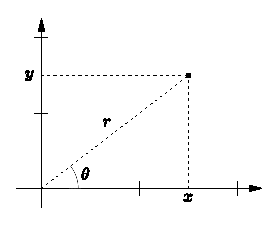
\includegraphics[scale=1.5]{resources/figura_01.eps}
    \caption{Coordenadas polares}\label{figura_01}
\end{figure}

\begin{equation*}
    \begin{cases}
        x=r\cos(\theta)\\
        y=r\sen(\theta)
    \end{cases}
\end{equation*}

\begin{equation*}
    T=\frac{1}{2}m(\dot{x}^2+\dot{y}^2)
\end{equation*}

Calculando la energía cinética en coordenadas polares:
n
\begin{equation*}
    \dot{x}=\dot{r}\cos(\theta)-r\sen(\theta)\dot{\theta}
\end{equation*}
\begin{equation*}
    \dot{y}=\dot{r}\sen(\theta)+r\cos(\theta)\dot{\theta}
\end{equation*}

\begin{equation*}
    \dot{x}^2=\dot{r}^2\cos^2(\theta)-
    2\dot{r}r\dot{\theta}\cos(\theta)\sen(\theta)+
    r^2\dot{\theta}^2\sen^2(\theta)
\end{equation*}
\begin{equation*}
    \dot{y}^2=\dot{r}^2\sen^2(\theta)+
    2\dot{r}r\dot{\theta}\sen(\theta)\cos(\theta)+
    r^2\dot{\theta}^2\cos^2(\theta)
\end{equation*}

\begin{equation*}
\begin{split}
    T&=\frac{1}{2}m(\dot{x}^2+\dot{y}^2)\\
     &=\frac{1}{2}m(\dot{r}^2\cos^2(\theta)+
       r^2\dot{\theta}^2\sen^2(\theta)+
       \dot{r}^2\sen^2(\theta)+
       r^2\dot{\theta}^2\cos^2(\theta))\\
     &=\frac{1}{2}m(\dot{r}^2(\cos^2(\theta)+
       \sen^2(\theta))+
       r^2\dot{\theta}^2(\sen^2(\theta)+
       \cos^2(\theta)))\\
     &=\frac{1}{2}m(\dot{r}^2+
       r^2\dot{\theta}^2)\\
\end{split}
\end{equation*}

\begin{equation}
\boxed{
    \begin{array}{l}
        T=\frac{1}{2}m(\dot{r}^2+r^2\dot{\theta}^2)
    \end{array}
}
\end{equation}

\subsection{Coordenadas cilíndricas}

\begin{figure}[H]
    \centering
    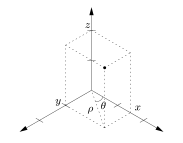
\includegraphics[scale=1.5]{resources/figura_02.eps}
    \caption{Coordenadas cilíndricas}\label{figura_02}
\end{figure}

\begin{equation*}
    \begin{cases}
        x=\rho\cos(\theta)\\
        y=\rho\sen(\theta)\\
        z=z
    \end{cases}
\end{equation*}

\begin{equation*}
    T=\frac{1}{2}m(\dot{x}^2+\dot{y}^2+\dot{z}^2)
\end{equation*}

Calculando la energía cinética en coordenadas cilíndricas:

\begin{equation*}
    \dot{x}=\dot{\rho}\cos(\theta)-\rho\sen(\theta)\dot{\theta}
\end{equation*}
\begin{equation*}
    \dot{y}=\dot{\rho}\sen(\theta)+\rho\cos(\theta)\dot{\theta}
\end{equation*}
\begin{equation*}
    \dot{z}=\dot{z}
\end{equation*}

\begin{equation*}
    \dot{x}^2=\dot{\rho}^2\cos^2(\theta)-
    2\dot{\rho}\rho\dot{\theta}\cos(\theta)\sen(\theta)+
    \rho^2\dot{\theta}^2\sen^2(\theta)
\end{equation*}
\begin{equation*}
    \dot{y}^2=\dot{\rho}^2\sen^2(\theta)+
    2\dot{\rho}\rho\dot{\theta}\sen(\theta)\cos(\theta)+
    \rho^2\dot{\theta}^2\cos^2(\theta)
\end{equation*}
\begin{equation*}
    \dot{z}^2=\dot{z}^2
\end{equation*}

\begin{equation*}
\begin{split}
    T&=\frac{1}{2}m(\dot{x}^2+\dot{y}^2+\dot{z}^2)\\
     &=\frac{1}{2}m(\dot{\rho}^2\cos^2(\theta)+
       \rho^2\dot{\theta}^2\sen^2(\theta)+
       \dot{\rho}^2\sen^2(\theta)+
       \rho^2\dot{\theta}^2\cos^2(\theta)+
       \dot{z}^2)\\
     &=\frac{1}{2}m(\dot{\rho}^2(\cos^2(\theta)+
       \sen^2(\theta))+
       \rho^2\dot{\theta}^2(\sen^2(\theta)+
       \cos^2(\theta))+
       \dot{z}^2)\\
     &=\frac{1}{2}m(\dot{\rho}^2+\rho^2\dot{\theta}^2+\dot{z}^2)\\
\end{split}
\end{equation*}

\begin{equation}
\boxed{
    \begin{array}{l}
        T=\frac{1}{2}m(\dot{\rho}^2+\rho^2\dot{\theta}^2+\dot{z}^2)
    \end{array}
}
\end{equation}

\subsection{Coordenadas esféricas}

\begin{figure}[H]
    \centering
    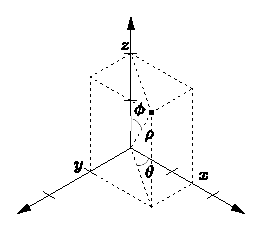
\includegraphics[scale=1.5]{resources/figura_03.eps}
    \caption{Coordenadas esféricas}\label{figura_03}
\end{figure}

\begin{equation*}
    \begin{cases}
        x=\rho\sen(\phi)\cos(\theta)\\
        y=\rho\sen(\phi)\sen(\theta)\\
        z=\rho\cos(\phi)
    \end{cases}
\end{equation*}

\begin{equation*}
    T=\frac{1}{2}m(\dot{x}^2+\dot{y}^2+\dot{z}^2)
\end{equation*}

Calculando la energía cinética en coordenadas esféricas:

\begin{equation*}
\begin{split}
    \dot{x}&=\dot{\rho}\sen(\phi)\cos(\theta)+
             \rho(\sen(\phi)\cos(\theta))'\\
           &=\dot{\rho}\sen(\phi)\cos(\theta)+
             \rho(\cos(\phi)\dot{\phi}\cos(\theta)+
             (-\sen(\theta))\dot{\theta}\sen(\phi))\\
           &=\dot{\rho}\sen(\phi)\cos(\theta)+
             \rho\dot{\phi}\cos(\phi)\cos(\theta)-
             \rho\dot{\theta}\sen(\theta)\sen(\phi)
\end{split}
\end{equation*}
\begin{equation*}
\begin{split}
    \dot{y}&=\dot{\rho}\sen(\phi)\sen(\theta)+
             \rho(\sen(\phi)\sen(\theta))'\\
           &=\dot{\rho}\sen(\phi)\sen(\theta)+
             \rho(\cos(\phi)\dot{\phi}\sen(\theta)+
             \cos(\theta)\dot{\theta}\sen(\phi))\\
           &=\dot{\rho}\sen(\phi)\sen(\theta)+
             \rho\dot{\phi}\cos(\phi)\sen(\theta)+
             \rho\dot{\theta}\cos(\theta)\sen(\phi)\\
\end{split}
\end{equation*}
\begin{equation*}
    \dot{z}=\dot{\rho}\cos(\phi)-\rho\dot{\phi}\sen(\phi)
\end{equation*}

\begin{equation*}
\begin{split}
    \dot{x}^2&=\dot{\rho}^2\sen^2(\phi)\cos^2(\theta)+
               \rho^2\dot{\phi}^2\cos^2(\phi)\cos^2(\theta)+
               \rho^2\dot{\theta}^2\sen^2(\theta)\sen^2(\phi)\\
             &+2\dot{\rho}\rho\dot{\phi}\sen(\phi)\cos^2(\theta)\cos(\phi)-
               2\rho^2\dot{\phi}\dot{\theta}
               \cos(\phi)\cos(\theta)\sen(\theta)\sen(\phi)-
               2\rho\dot{\rho}\dot{\theta}
               \sen^2(\phi)\cos(\theta)\sen(\theta)\\
\end{split}
\end{equation*}
\begin{equation*}
\begin{split}
    \dot{y}^2&=\dot{\rho}^2\sen^2(\phi)\sen^2(\theta)+
               \rho^2\dot{\phi}^2\cos^2(\phi)\sen^2(\theta)+
               \rho^2\dot{\theta}^2\cos^2(\theta)\sen^2(\phi)\\
             &+2\dot{\rho}\rho\dot{\phi}\sen(\phi)\sen^2(\theta)\cos(\phi)+
               2\rho^2\dot{\phi}\dot{\theta}
               \cos(\phi)\sen(\theta)\cos(\theta)\sen(\phi)+
               2\rho\dot{\theta}\dot{\rho}
               \cos(\theta)\sen^2(\phi)\sen(\theta)
\end{split}
\end{equation*}
\begin{equation*}
    \dot{z}^2=\dot{\rho}^2\cos^2(\phi)-
              2\dot{\rho}\rho\dot{\phi}\cos(\phi)\sen(\phi)+
              \rho^2\dot{\phi}^2\sen^2(\phi)
\end{equation*}

\begin{equation*}
\begin{split}
    T&=\frac{1}{2}m(\dot{x}^2+\dot{y}^2+\dot{z}^2)\\
     &=\frac{1}{2}m(\dot{\rho}^2\sen^2(\phi)+
       \rho^2\dot{\phi}^2\cos^2(\phi)+
       \rho^2\dot{\theta}^2\sen^2(\phi)\\
     &+2\dot{\rho}\rho\dot{\phi}\sen(\phi)\cos(\phi)+
       \dot{\rho}^2\cos^2(\phi)-
       2\dot{\rho}\rho\dot{\phi}\cos(\phi)\sen(\phi)+
       \rho^2\dot{\phi}^2\sen^2(\phi))\\
     &=\frac{1}{2}m(\dot{\rho}^2+
       \rho^2\dot{\phi}^2+
       \rho^2\dot{\theta}^2\sen^2(\phi))
\end{split}
\end{equation*}

\begin{equation}
\boxed{
    \begin{array}{l}
        T=\frac{1}{2}m(\dot{\rho}^2+
        \rho^2\dot{\phi}^2+
        \rho^2\dot{\theta}^2\sen^2(\phi))
    \end{array}
}
\end{equation}


\chapter{Análisis de formas de onda periódica}

\section{Funciones pares e impares}
Una función es \textbf{par} si:
\begin{equation}
    f(-t)=f(t)
\end{equation}
\begin{figure}[H]
    \centering
    \input{figura_02_01.tex}
    \caption{La gráfica se refleja \\respecto al eje central.}
\end{figure}

\textbf{Ejemplo 1:}
\begin{equation*}
    f(t)=t^2
\end{equation*}
\begin{equation*}
    f(-t)={(-t)}^2=t^2=f(t)
\end{equation*}

\textbf{Ejemplo 2:}
\begin{equation*}
    f(t)=\cos(t)
\end{equation*}
\begin{equation*}
    f(t)=\cos(-t)=\cos(t)=f(t)
\end{equation*}

Una función es \textbf{impar} si:
\begin{equation}
    f(-t)=-f(t)
\end{equation}
\begin{figure}[H]
    \centering
    % GNUPLOT: LaTeX picture with Postscript
\begingroup
  \makeatletter
  \providecommand\color[2][]{%
    \GenericError{(gnuplot) \space\space\space\@spaces}{%
      Package color not loaded in conjunction with
      terminal option `colourtext'%
    }{See the gnuplot documentation for explanation.%
    }{Either use 'blacktext' in gnuplot or load the package
      color.sty in LaTeX.}%
    \renewcommand\color[2][]{}%
  }%
  \providecommand\includegraphics[2][]{%
    \GenericError{(gnuplot) \space\space\space\@spaces}{%
      Package graphicx or graphics not loaded%
    }{See the gnuplot documentation for explanation.%
    }{The gnuplot epslatex terminal needs graphicx.sty or graphics.sty.}%
    \renewcommand\includegraphics[2][]{}%
  }%
  \providecommand\rotatebox[2]{#2}%
  \@ifundefined{ifGPcolor}{%
    \newif\ifGPcolor
    \GPcolorfalse
  }{}%
  \@ifundefined{ifGPblacktext}{%
    \newif\ifGPblacktext
    \GPblacktexttrue
  }{}%
  % define a \g@addto@macro without @ in the name:
  \let\gplgaddtomacro\g@addto@macro
  % define empty templates for all commands taking text:
  \gdef\gplbacktext{}%
  \gdef\gplfronttext{}%
  \makeatother
  \ifGPblacktext
    % no textcolor at all
    \def\colorrgb#1{}%
    \def\colorgray#1{}%
  \else
    % gray or color?
    \ifGPcolor
      \def\colorrgb#1{\color[rgb]{#1}}%
      \def\colorgray#1{\color[gray]{#1}}%
      \expandafter\def\csname LTw\endcsname{\color{white}}%
      \expandafter\def\csname LTb\endcsname{\color{black}}%
      \expandafter\def\csname LTa\endcsname{\color{black}}%
      \expandafter\def\csname LT0\endcsname{\color[rgb]{1,0,0}}%
      \expandafter\def\csname LT1\endcsname{\color[rgb]{0,1,0}}%
      \expandafter\def\csname LT2\endcsname{\color[rgb]{0,0,1}}%
      \expandafter\def\csname LT3\endcsname{\color[rgb]{1,0,1}}%
      \expandafter\def\csname LT4\endcsname{\color[rgb]{0,1,1}}%
      \expandafter\def\csname LT5\endcsname{\color[rgb]{1,1,0}}%
      \expandafter\def\csname LT6\endcsname{\color[rgb]{0,0,0}}%
      \expandafter\def\csname LT7\endcsname{\color[rgb]{1,0.3,0}}%
      \expandafter\def\csname LT8\endcsname{\color[rgb]{0.5,0.5,0.5}}%
    \else
      % gray
      \def\colorrgb#1{\color{black}}%
      \def\colorgray#1{\color[gray]{#1}}%
      \expandafter\def\csname LTw\endcsname{\color{white}}%
      \expandafter\def\csname LTb\endcsname{\color{black}}%
      \expandafter\def\csname LTa\endcsname{\color{black}}%
      \expandafter\def\csname LT0\endcsname{\color{black}}%
      \expandafter\def\csname LT1\endcsname{\color{black}}%
      \expandafter\def\csname LT2\endcsname{\color{black}}%
      \expandafter\def\csname LT3\endcsname{\color{black}}%
      \expandafter\def\csname LT4\endcsname{\color{black}}%
      \expandafter\def\csname LT5\endcsname{\color{black}}%
      \expandafter\def\csname LT6\endcsname{\color{black}}%
      \expandafter\def\csname LT7\endcsname{\color{black}}%
      \expandafter\def\csname LT8\endcsname{\color{black}}%
    \fi
  \fi
    \setlength{\unitlength}{0.0500bp}%
    \ifx\gptboxheight\undefined%
      \newlength{\gptboxheight}%
      \newlength{\gptboxwidth}%
      \newsavebox{\gptboxtext}%
    \fi%
    \setlength{\fboxrule}{0.5pt}%
    \setlength{\fboxsep}{1pt}%
    \definecolor{tbcol}{rgb}{1,1,1}%
\begin{picture}(4320.00,2880.00)%
    \gplgaddtomacro\gplbacktext{%
      \csname LTb\endcsname%%
      \put(2040,192){\makebox(0,0)[r]{\strut{}}}%
      \put(2040,824){\makebox(0,0)[r]{\strut{}}}%
      \put(2040,1456){\makebox(0,0)[r]{\strut{}}}%
      \put(2040,2087){\makebox(0,0)[r]{\strut{}}}%
      \put(2040,2719){\makebox(0,0)[r]{\strut{}}}%
      \put(240,1233){\makebox(0,0){\strut{}}}%
      \put(714,1233){\makebox(0,0){\strut{}}}%
      \put(1188,1233){\makebox(0,0){\strut{}}}%
      \put(1662,1233){\makebox(0,0){\strut{}}}%
      \put(2136,1233){\makebox(0,0){\strut{}}}%
      \put(2609,1233){\makebox(0,0){\strut{}}}%
      \put(3083,1233){\makebox(0,0){\strut{}}}%
      \put(3557,1233){\makebox(0,0){\strut{}}}%
      \put(4031,1233){\makebox(0,0){\strut{}}}%
      \csname LTb\endcsname%%
      \put(4647,1456){\makebox(0,0)[l]{\strut{}$t$}}%
      \put(2349,2845){\makebox(0,0)[l]{\strut{}$f(t)$}}%
      \put(998,1645){\makebox(0,0)[l]{\strut{}$-t_1$}}%
      \put(3036,1266){\makebox(0,0)[l]{\strut{}$ t_1$}}%
      \put(2372,824){\makebox(0,0)[l]{\strut{}$-f(t_1)=f(-t_1)$}}%
    }%
    \gplgaddtomacro\gplfronttext{%
    }%
    \gplbacktext
    \put(0,0){\includegraphics[width={216.00bp},height={144.00bp}]{figura_02_02}}%
    \gplfronttext
  \end{picture}%
\endgroup

    \caption{La gráfica se refleja \\
    1ro respecto al eje central\\
    2do respecto al eje horizontal.}
\end{figure}

\textbf{Ejemplo 3:}
\begin{equation*}
    f(t)=t^3
\end{equation*}
\begin{equation*}
    f(-t)={(-t)}^3=-t^3=-f(t)
\end{equation*}

\textbf{Ejemplo 4:}
\begin{equation*}
    f(t)=\sen(t)
\end{equation*}
\begin{equation*}
    f(t)=\sen(-t)=-\sen(t)=-f(t)
\end{equation*}

\textbf{Ejemplo 5:}
\begin{equation*}
    f(t)=\begin{cases}
        e^t&t<0\\
        e^{-t}&t>0\\
    \end{cases}
\end{equation*}
\begin{equation*}
    f(-t)=\left\{\!\begin{aligned}
    &e^{-t}&-t<0\rightarrow\,t>0\\
    &e^{t}&-t>0\rightarrow\,t<0\\
    \end{aligned}\right\}
    =f(t)
\end{equation*}
\begin{figure}[H]
    \centering
    % GNUPLOT: LaTeX picture with Postscript
\begingroup
  \makeatletter
  \providecommand\color[2][]{%
    \GenericError{(gnuplot) \space\space\space\@spaces}{%
      Package color not loaded in conjunction with
      terminal option `colourtext'%
    }{See the gnuplot documentation for explanation.%
    }{Either use 'blacktext' in gnuplot or load the package
      color.sty in LaTeX.}%
    \renewcommand\color[2][]{}%
  }%
  \providecommand\includegraphics[2][]{%
    \GenericError{(gnuplot) \space\space\space\@spaces}{%
      Package graphicx or graphics not loaded%
    }{See the gnuplot documentation for explanation.%
    }{The gnuplot epslatex terminal needs graphicx.sty or graphics.sty.}%
    \renewcommand\includegraphics[2][]{}%
  }%
  \providecommand\rotatebox[2]{#2}%
  \@ifundefined{ifGPcolor}{%
    \newif\ifGPcolor
    \GPcolorfalse
  }{}%
  \@ifundefined{ifGPblacktext}{%
    \newif\ifGPblacktext
    \GPblacktexttrue
  }{}%
  % define a \g@addto@macro without @ in the name:
  \let\gplgaddtomacro\g@addto@macro
  % define empty templates for all commands taking text:
  \gdef\gplbacktext{}%
  \gdef\gplfronttext{}%
  \makeatother
  \ifGPblacktext
    % no textcolor at all
    \def\colorrgb#1{}%
    \def\colorgray#1{}%
  \else
    % gray or color?
    \ifGPcolor
      \def\colorrgb#1{\color[rgb]{#1}}%
      \def\colorgray#1{\color[gray]{#1}}%
      \expandafter\def\csname LTw\endcsname{\color{white}}%
      \expandafter\def\csname LTb\endcsname{\color{black}}%
      \expandafter\def\csname LTa\endcsname{\color{black}}%
      \expandafter\def\csname LT0\endcsname{\color[rgb]{1,0,0}}%
      \expandafter\def\csname LT1\endcsname{\color[rgb]{0,1,0}}%
      \expandafter\def\csname LT2\endcsname{\color[rgb]{0,0,1}}%
      \expandafter\def\csname LT3\endcsname{\color[rgb]{1,0,1}}%
      \expandafter\def\csname LT4\endcsname{\color[rgb]{0,1,1}}%
      \expandafter\def\csname LT5\endcsname{\color[rgb]{1,1,0}}%
      \expandafter\def\csname LT6\endcsname{\color[rgb]{0,0,0}}%
      \expandafter\def\csname LT7\endcsname{\color[rgb]{1,0.3,0}}%
      \expandafter\def\csname LT8\endcsname{\color[rgb]{0.5,0.5,0.5}}%
    \else
      % gray
      \def\colorrgb#1{\color{black}}%
      \def\colorgray#1{\color[gray]{#1}}%
      \expandafter\def\csname LTw\endcsname{\color{white}}%
      \expandafter\def\csname LTb\endcsname{\color{black}}%
      \expandafter\def\csname LTa\endcsname{\color{black}}%
      \expandafter\def\csname LT0\endcsname{\color{black}}%
      \expandafter\def\csname LT1\endcsname{\color{black}}%
      \expandafter\def\csname LT2\endcsname{\color{black}}%
      \expandafter\def\csname LT3\endcsname{\color{black}}%
      \expandafter\def\csname LT4\endcsname{\color{black}}%
      \expandafter\def\csname LT5\endcsname{\color{black}}%
      \expandafter\def\csname LT6\endcsname{\color{black}}%
      \expandafter\def\csname LT7\endcsname{\color{black}}%
      \expandafter\def\csname LT8\endcsname{\color{black}}%
    \fi
  \fi
    \setlength{\unitlength}{0.0500bp}%
    \ifx\gptboxheight\undefined%
      \newlength{\gptboxheight}%
      \newlength{\gptboxwidth}%
      \newsavebox{\gptboxtext}%
    \fi%
    \setlength{\fboxrule}{0.5pt}%
    \setlength{\fboxsep}{1pt}%
    \definecolor{tbcol}{rgb}{1,1,1}%
\begin{picture}(5760.00,1440.00)%
    \gplgaddtomacro\gplbacktext{%
      \csname LTb\endcsname%%
      \put(2760,464){\makebox(0,0)[r]{\strut{}}}%
      \put(2760,1007){\makebox(0,0)[r]{\strut{}}}%
      \put(240,241){\makebox(0,0){\strut{}}}%
      \put(763,241){\makebox(0,0){\strut{}}}%
      \put(1286,241){\makebox(0,0){\strut{}}}%
      \put(1809,241){\makebox(0,0){\strut{}}}%
      \put(2332,241){\makebox(0,0){\strut{}}}%
      \put(2856,241){\makebox(0,0){\strut{}}}%
      \put(3379,241){\makebox(0,0){\strut{}}}%
      \put(3902,241){\makebox(0,0){\strut{}}}%
      \put(4425,241){\makebox(0,0){\strut{}}}%
      \put(4948,241){\makebox(0,0){\strut{}}}%
      \put(5471,241){\makebox(0,0){\strut{}}}%
      \csname LTb\endcsname%%
      \put(6256,464){\makebox(0,0)[l]{\strut{}$t$}}%
      \put(2751,1496){\makebox(0,0)[l]{\strut{}$f(t)$}}%
    }%
    \gplgaddtomacro\gplfronttext{%
    }%
    \gplgaddtomacro\gplbacktext{%
      \csname LTb\endcsname%%
      \put(2760,464){\makebox(0,0)[r]{\strut{}}}%
      \put(2760,1007){\makebox(0,0)[r]{\strut{}}}%
      \put(240,241){\makebox(0,0){\strut{}}}%
      \put(763,241){\makebox(0,0){\strut{}}}%
      \put(1286,241){\makebox(0,0){\strut{}}}%
      \put(1809,241){\makebox(0,0){\strut{}}}%
      \put(2332,241){\makebox(0,0){\strut{}}}%
      \put(2856,241){\makebox(0,0){\strut{}}}%
      \put(3379,241){\makebox(0,0){\strut{}}}%
      \put(3902,241){\makebox(0,0){\strut{}}}%
      \put(4425,241){\makebox(0,0){\strut{}}}%
      \put(4948,241){\makebox(0,0){\strut{}}}%
      \put(5471,241){\makebox(0,0){\strut{}}}%
      \csname LTb\endcsname%%
      \put(6256,464){\makebox(0,0)[l]{\strut{}$t$}}%
      \put(2751,1496){\makebox(0,0)[l]{\strut{}$f(t)$}}%
    }%
    \gplgaddtomacro\gplfronttext{%
    }%
    \gplbacktext
    \put(0,0){\includegraphics[width={288.00bp},height={72.00bp}]{figura_02_03}}%
    \gplfronttext
  \end{picture}%
\endgroup

\end{figure}

\subsection{Propiedades de las funciones pares e impares}
\subsubsection*{Propiedad 1}
Si $f(t)$ es \textbf{par} y $g(t)$ es \textbf{par}, entonces $h(t)=f(t)g(t)$ es
\textbf{par}.

\underline{Prueba}:
\begin{equation*}
\begin{cases}
    &f(-t)=f(t)\\
    &g(-t)=g(t)\\
\end{cases}
\end{equation*}
\begin{equation*}
\begin{split}
    h(-t)
        &=f(-t)g(-t)\\
        &=f(t)g(t)\\
        &=h(t)\\
\end{split}
\end{equation*}

\subsubsection*{Propiedad 2}
Si $f(t)$ es \textbf{impar} y $g(t)$ es \textbf{impar}, entonces $h(t)=f(t)g(t)$
es \textbf{par}.

\underline{Prueba}:
\begin{equation*}
\begin{cases}
    &f(-t)=-f(t)\\
    &g(-t)=-g(t)\\
\end{cases}
\end{equation*}

\subsubsection*{Propiedad 3}
Si $f(t)$ es \textbf{par} y $g(t)$ es \textbf{impar}, entonces $h(t)=f(t)g(t)$
es \textbf{impar}.

\underline{Prueba}:
\begin{equation*}
\begin{cases}
    &f(-t)=f(t)\\
    &g(-t)=-g(t)\\
\end{cases}
\end{equation*}
\begin{equation*}
\begin{split}
    h(-t)
        &=f(-t)g(-t)\\
        &=f(t)(-g(t))\\
        &=-f(t)g(t)\\
        &=-h(t)\\
\end{split}
\end{equation*}

\subsubsection*{Propiedad 4}
Si $f(t)$ es \textbf{par}, entonces:
\begin{equation}
    \int_{-a}^a\,f(t)\,dt=2\int_0^a\,f(t)\,dt
\end{equation}
\begin{figure}[H]
    \centering
    \input{figura_02_04.tex}
\end{figure}

\underline{Prueba}:
\begin{equation*}
\begin{split}
    \int_{-a}^a\,f(t)\,dt
        &=\int_{-a}^0\,f(t)\,dt+\int_0^a\,f(t)\,dt\\
        &=\int_{-a}^0\,f(-t)\,dt+\int_0^a\,f(t)\,dt\\
\end{split}
\end{equation*}
\begin{equation*}
    \tau=-t
\end{equation*}
\begin{equation*}
    d\tau=-dt
\end{equation*}
\begin{equation*}
\begin{split}
    \int_{-a}^a\,f(t)\,dt
        &=\int_a^0\,f(\tau)\,(-d\tau)+\int_0^a\,f(t)\,dt\\
        &=\int_0^a\,f(\tau)\,d\tau+\int_0^a\,f(t)\,dt\\
        &=2\int_0^a\,f(t)\,dt\\
\end{split}
\end{equation*}

\subsubsection*{Propiedad 5}
Si $f(t)$ es \textbf{impar}, entonces:
\begin{equation}
    \int_{-a}^a\,f(t)\,dt=0
\end{equation}
\begin{figure}[H]
    \centering
    \input{figura_02_05.tex}
\end{figure}

\underline{Prueba}:
\begin{equation*}
\begin{split}
    \int_{-a}^a\,f(t)\,dt
        &=\int_{-a}^0\,f(t)\,dt+\int_0^a\,f(t)\,dt\\
        &=\int_{-a}^0\,-f(-t)\,dt+\int_0^a\,f(t)\,dt\\
\end{split}
\end{equation*}
\begin{equation*}
    \tau=-t
\end{equation*}
\begin{equation*}
    d\tau=-dt
\end{equation*}
\begin{equation*}
\begin{split}
    \int_{-a}^a\,f(t)\,dt
        &=-\int_a^0\,f(\tau)\,(-d\tau)+\int_0^a\,f(t)\,dt\\
        &=-\int_0^a\,f(\tau)\,d\tau+\int_0^a\,f(t)\,dt\\
        &=0\\
\end{split}
\end{equation*}

\subsection{Evaluación de coeficientes de \emph{Fourier}}
\subsubsection{Simetría par}
\begin{equation*}
\begin{split}
    a_0
        &=\frac{2}{T}\int_0^T\,f(t)\,dt\\
        &=\frac{2}{T}\int_{-T/2}^{T/2}\,f(t)\,dt\\
        &=\frac{2}{T}\left(2\int_0^{T/2}\,f(t)\,dt\right)\\
        &=\frac{4}{T}\int_0^{T/2}\,f(t)\,dt\\
\end{split}
\end{equation*}
\begin{equation}
    a_0=\frac{4}{T}\int_0^{T/2}\,f(t)\,dt
\end{equation}
\begin{equation*}
\begin{split}
    a_n
        &=\frac{2}{T}\int_{-T/2}^{T/2}f(t)\cos(n\omega_0\,t)\,dt\\
        &=\frac{2}{T}\left(2\int_0^{T/2}f(t)\cos(n\omega_0\,t)\,dt\right)\\
        &=\frac{4}{T}\int_0^{T/2}f(t)\cos(n\omega_0\,t)\,dt\\
\end{split}
\end{equation*}
\begin{equation}
    a_n=\frac{4}{T}\int_0^{T/2}f(t)\cos(n\omega_0\,t)\,dt
\end{equation}
\begin{equation*}
\begin{split}
    b_n
        &=\frac{2}{T}\int_{-T/2}^{T/2}f(t)\sen(n\omega_0\,t)\,dt\\
        &=0\\
\end{split}
\end{equation*}
\begin{equation}
    b_n=0
\end{equation}

\subsubsection{Simetría impar}
\begin{equation*}
\begin{split}
    a_0
        &=\frac{2}{T}\int_0^T\,f(t)\,dt\\
        &=\frac{2}{T}\int_{-T/2}^{T/2}\,f(t)\,dt\\
        &=0\\
\end{split}
\end{equation*}
\begin{equation}
    a_0=0
\end{equation}
\begin{equation*}
\begin{split}
    a_n
        &=\frac{2}{T}\int_{-T/2}^{T/2}\,f(t)\cos(n\omega_0\,t)\,dt\\
        &=0\\
\end{split}
\end{equation*}
\begin{equation}
    a_n=0
\end{equation}
\begin{equation*}
\begin{split}
    b_n
        &=\frac{2}{T}\int_{-T/2}^{T/2}\,f(t)\sen(n\omega_0\,t)\,dt\\
        &=\frac{2}{T}\left(2\int_0^{T/2}\,f(t)\sen(n\omega_0\,t)\,dt\right)\\
        &=\frac{4}{T}\int_0^{T/2}f(t)\sen(n\omega_0\,t)\,dt\\
\end{split}
\end{equation*}
\begin{equation}
    b_n=\frac{4}{T}\int_0^{T/2}f(t)\sen(n\omega_0\,t)\,dt
\end{equation}

\section{Simetría de media onda (S.M.O.)}
$f(t)$ tiene simetría de media onda si:
\begin{equation*}
    f(t)=-f(t\pm\frac{T}{2})
\end{equation*}
\begin{figure}[H]
    \centering
    \input{figura_02_06.tex}
    \caption{La gráfica se desplaza $1/2$ periodo\\
    y se refleja respecto a $t$.}
\end{figure}

\subsection{Evaluación de coeficientes de \emph{Fourier}}
\begin{equation*}
\begin{split}
    a_0
        &=\frac{2}{T}\int_0^T\,f(t)\,dt\\
        &=\frac{2}{T}\left[\int_0^{T/2}f(t)\,dt+\int_{T/2}^T\,f(t)\,dt\right]\\
        &=\frac{2}{T}\left[
            \int_0^{T/2}f(t)\,dt-\int_{t=T/2}^{t=T}f(t-\frac{T}{2})\,dt
        \right]\\
\end{split}
\end{equation*}
\begin{equation*}
    \tau=t-\frac{T}{2}
\end{equation*}
\begin{equation*}
    d\tau=dt
\end{equation*}
\begin{equation*}
\begin{split}
    a_0
        &=\frac{2}{T}\left[
            \int_0^{T/2}f(t)\,dt-
            \int_{\tau=T/2-T/2}^{\tau=T-T/2}f(\tau)\,d\tau
        \right]\\
        &=\frac{2}{T}\left[
            \int_0^{T/2}f(t)\,dt-\int_0^{T/2}f(\tau)\,d\tau
        \right]\\
\end{split}
\end{equation*}
\begin{equation}
    a_0=0
\end{equation}
\begin{equation*}
\begin{split}
    a_n
        &=\frac{2}{T}\int_0^T\,f(t)\cos(n\omega_0\,t)\,dt\\
        &=\frac{2}{T}\left[
            \int_0^{T/2}f(t)\cos(n\omega_0\,t)\,dt+
            \int_{T/2}^T\,f(t)\cos(n\omega_0\,t)\,dt
        \right]\\
        &=\frac{2}{T}\left[
            \int_0^{T/2}f(t)\cos(n\omega_0\,t)\,dt-
            \int_{T/2}^T\,f(t-\frac{T}{2})\cos(n\omega_0\,t)\,dt
        \right]\\
\end{split}
\end{equation*}
\begin{equation*}
    \tau=t-\frac{T}{2}
\end{equation*}
\begin{equation*}
    d\tau=dt
\end{equation*}
\begin{equation*}
\begin{split}
    a_n
        &=\frac{2}{T}\left[
            \int_0^{T/2}f(t)\cos(n\omega_0\,t)\,dt-
            \int_{\tau=T/2-T/2}^{\tau=T-T/2}
                f(\tau)\cos(n\omega_0(\tau+\frac{T}{2}))\,d\tau
        \right]\\
        &=\frac{2}{T}\left[
            \int_0^{T/2}f(t)\cos(n\omega_0\,t)\,dt-
            \int_0^{T/2}f(\tau)\cos(n\omega_0(\tau+\frac{T}{2}))\,d\tau
        \right]\\
\end{split}
\end{equation*}
\begin{equation*}
\begin{split}
    n\omega_0(\tau+T/2)
        &=n\omega_0\tau+n\omega_0\frac{T}{2}\\
        &=n\omega_0\tau+n\frac{2\pi}{T}\frac{T}{2}\\
        &=n\omega_0\tau+n\pi\\
\end{split}
\end{equation*}
\begin{equation*}
\begin{split}
    \cos(n\omega_0\tau+n\pi)
        &=\cos(n\omega_0\tau)\cos(n\pi)-\sen(n\pi)\sen(n\omega_0\tau)\\
        &=\cos(n\omega_0\tau)\cos(n\pi)\\
\end{split}
\end{equation*}
\begin{equation*}
\begin{split}
    a_n
        &=\frac{2}{T}\left[
            \int_0^{T/2}f(t)\cos(n\omega_0\,t)\,dt-
            \int_0^{T/2}f(\tau)\cos(n\omega_0\tau)\cos(n\pi)\,d\tau
        \right]\\
        &=\frac{2}{T}\left[
            \int_0^{T/2}f(t)\cos(n\omega_0\,t)\,dt-\cos(n\pi)\int_0^{T/2}
                f(\tau)\cos(n\omega_0\tau)\,d\tau
        \right]\\
        &=\frac{2}{T}(1-\cos(\pi\,n))\left(
            \int_0^{T/2}f(t)\cos(n\omega_0\,t)\,dt
        \right)\\
\end{split}
\end{equation*}
\begin{equation*}
    \cos(\pi\,n)=\begin{cases}
        1&n:\text{par}\\
        -1&n:\text{impar}\\
    \end{cases}
\end{equation*}
\begin{equation}
\begin{cases}
    n:\text{par}&a_n=0\\
    n:\text{impar}&a_n=\frac{4}{T}\int_0^{T/2}f(t)\cos(n\omega_0\,t)\,dt\\
\end{cases}
\end{equation}
\begin{equation*}
\begin{split}
    b_n
        &=\frac{2}{T}\int_0^T\,f(t)\sen(n\omega_0\,t)\,dt\\
        &=\frac{2}{T}\left[
            \int_0^{T/2}\,f(t)\sen(n\omega_0\,t)\,dt+
            \int_{T/2}^T\,f(t)\sen(n\omega_0\,t)\,dt
        \right]\\
        &=\frac{2}{T}\left[
            \int_0^{T/2}\,f(t)\sen(n\omega_0\,t)\,dt-
            \int_{T/2}^T\,f(t-\frac{T}{2})\sen(n\omega_0\,t)\,dt
        \right]\\
\end{split}
\end{equation*}
\begin{equation*}
    \tau=t-\frac{T}{2}
\end{equation*}
\begin{equation*}
    d\tau=dt
\end{equation*}
\begin{equation*}
\begin{split}
    b_n
        &=\frac{2}{T}\left[
            \int_0^{T/2}\,f(t)\sen(n\omega_0\,t)\,dt-
            \int_{\tau=T/2-T/2}^{\tau=T-T/2}
                f(\tau)\sen(n\omega_0(\tau+\frac{T}{2}))\,d\tau
        \right]\\
        &=\frac{2}{T}\left[
            \int_0^{T/2}\,f(t)\sen(n\omega_0\,t)\,dt-
            \int_0^{T/2}\,f(\tau)\sen(n\omega_0(\tau+\frac{T}{2}))\,d\tau
        \right]\\
\end{split}
\end{equation*}
\begin{equation*}
\begin{split}
    n\omega_0(\tau+T/2)
        &=n\omega_0\tau+n\omega_0\frac{T}{2}\\
        &=n\omega_0\tau+n\frac{2\pi}{T}\frac{T}{2}\\
        &=n\omega_0\tau+n\pi\\
\end{split}
\end{equation*}
\begin{equation*}
\begin{split}
    \sen(n\omega_0\tau+n\pi)
        &=\sen(n\omega_0\tau)\cos(n\pi)+\sen(n\pi)\cos(n\omega_0\tau)\\
        &=\sen(n\omega_0\tau)\cos(n\pi)\\
\end{split}
\end{equation*}
\begin{equation*}
\begin{split}
    b_n
        &=\frac{2}{T}\left[
            \int_0^{T/2}\,f(t)\sen(n\omega_0\,t)\,dt-
            \int_0^{T/2}\,f(\tau)\sen(n\omega_0\tau)\cos(n\pi)\,d\tau
        \right]\\
        &=\frac{2}{T}\left[
            \int_0^{T/2}\,f(t)\sen(n\omega_0\,t)\,dt-
            \cos(n\pi)\int_0^{T/2}\,f(\tau)\sen(n\omega_0\tau)\,d\tau
        \right]\\
        &=\frac{2}{T}(1-\cos(\pi\,n))\left(
            \int_0^{T/2}\,f(t)\sen(n\omega_0\,t)\,dt
        \right)\\
\end{split}
\end{equation*}
\begin{equation*}
    \cos(\pi\,n)=\begin{cases}
        1&n:\text{par}\\
        -1&n:\text{impar}\\
    \end{cases}
\end{equation*}
\begin{equation}
\begin{cases}
    n:\text{par}&b_n=0\\
    n:\text{impar}&b_n=\frac{4}{T}\int_0^{T/2}f(t)\sen(n\omega_0\,t)\,dt\\
\end{cases}
\end{equation}

\section{Simetría de cuarto de onda (S.C.O.)}
\subsection{Simetría de cuarto de onda par}
Una función $f(t)$ tiene simetría de cuarto de onda \textbf{par} cuando:
\begin{itemize}
    \item $f(t)$ es \textbf{par}.
    \item $f(t)$ tiene simetría de media onda.
\end{itemize}
\begin{figure}[H]
    \centering
    \input{figura_02_07.tex}
\end{figure}

\subsection{Simetría de cuarto de onda impar}
Una función $f(t)$ tiene simetría de cuarto de onda \textbf{impar} cuando:
\begin{itemize}
    \item $f(t)$ es \textbf{impar}.
    \item $f(t)$ tiene simetría de media onda.
\end{itemize}
\begin{figure}[H]
    \centering
    % GNUPLOT: LaTeX picture with Postscript
\begingroup
  \makeatletter
  \providecommand\color[2][]{%
    \GenericError{(gnuplot) \space\space\space\@spaces}{%
      Package color not loaded in conjunction with
      terminal option `colourtext'%
    }{See the gnuplot documentation for explanation.%
    }{Either use 'blacktext' in gnuplot or load the package
      color.sty in LaTeX.}%
    \renewcommand\color[2][]{}%
  }%
  \providecommand\includegraphics[2][]{%
    \GenericError{(gnuplot) \space\space\space\@spaces}{%
      Package graphicx or graphics not loaded%
    }{See the gnuplot documentation for explanation.%
    }{The gnuplot epslatex terminal needs graphicx.sty or graphics.sty.}%
    \renewcommand\includegraphics[2][]{}%
  }%
  \providecommand\rotatebox[2]{#2}%
  \@ifundefined{ifGPcolor}{%
    \newif\ifGPcolor
    \GPcolorfalse
  }{}%
  \@ifundefined{ifGPblacktext}{%
    \newif\ifGPblacktext
    \GPblacktexttrue
  }{}%
  % define a \g@addto@macro without @ in the name:
  \let\gplgaddtomacro\g@addto@macro
  % define empty templates for all commands taking text:
  \gdef\gplbacktext{}%
  \gdef\gplfronttext{}%
  \makeatother
  \ifGPblacktext
    % no textcolor at all
    \def\colorrgb#1{}%
    \def\colorgray#1{}%
  \else
    % gray or color?
    \ifGPcolor
      \def\colorrgb#1{\color[rgb]{#1}}%
      \def\colorgray#1{\color[gray]{#1}}%
      \expandafter\def\csname LTw\endcsname{\color{white}}%
      \expandafter\def\csname LTb\endcsname{\color{black}}%
      \expandafter\def\csname LTa\endcsname{\color{black}}%
      \expandafter\def\csname LT0\endcsname{\color[rgb]{1,0,0}}%
      \expandafter\def\csname LT1\endcsname{\color[rgb]{0,1,0}}%
      \expandafter\def\csname LT2\endcsname{\color[rgb]{0,0,1}}%
      \expandafter\def\csname LT3\endcsname{\color[rgb]{1,0,1}}%
      \expandafter\def\csname LT4\endcsname{\color[rgb]{0,1,1}}%
      \expandafter\def\csname LT5\endcsname{\color[rgb]{1,1,0}}%
      \expandafter\def\csname LT6\endcsname{\color[rgb]{0,0,0}}%
      \expandafter\def\csname LT7\endcsname{\color[rgb]{1,0.3,0}}%
      \expandafter\def\csname LT8\endcsname{\color[rgb]{0.5,0.5,0.5}}%
    \else
      % gray
      \def\colorrgb#1{\color{black}}%
      \def\colorgray#1{\color[gray]{#1}}%
      \expandafter\def\csname LTw\endcsname{\color{white}}%
      \expandafter\def\csname LTb\endcsname{\color{black}}%
      \expandafter\def\csname LTa\endcsname{\color{black}}%
      \expandafter\def\csname LT0\endcsname{\color{black}}%
      \expandafter\def\csname LT1\endcsname{\color{black}}%
      \expandafter\def\csname LT2\endcsname{\color{black}}%
      \expandafter\def\csname LT3\endcsname{\color{black}}%
      \expandafter\def\csname LT4\endcsname{\color{black}}%
      \expandafter\def\csname LT5\endcsname{\color{black}}%
      \expandafter\def\csname LT6\endcsname{\color{black}}%
      \expandafter\def\csname LT7\endcsname{\color{black}}%
      \expandafter\def\csname LT8\endcsname{\color{black}}%
    \fi
  \fi
    \setlength{\unitlength}{0.0500bp}%
    \ifx\gptboxheight\undefined%
      \newlength{\gptboxheight}%
      \newlength{\gptboxwidth}%
      \newsavebox{\gptboxtext}%
    \fi%
    \setlength{\fboxrule}{0.5pt}%
    \setlength{\fboxsep}{1pt}%
    \definecolor{tbcol}{rgb}{1,1,1}%
\begin{picture}(7200.00,3456.00)%
    \gplgaddtomacro\gplbacktext{%
      \csname LTb\endcsname%%
      \put(3480,192){\makebox(0,0)[r]{\strut{}}}%
      \put(3480,709){\makebox(0,0)[r]{\strut{}}}%
      \put(3480,1226){\makebox(0,0)[r]{\strut{}}}%
      \put(3480,1744){\makebox(0,0)[r]{\strut{}}}%
      \put(3480,2261){\makebox(0,0)[r]{\strut{}}}%
      \put(3480,2778){\makebox(0,0)[r]{\strut{}}}%
      \put(3480,3295){\makebox(0,0)[r]{\strut{}}}%
      \put(240,1521){\makebox(0,0){\strut{}}}%
      \put(907,1521){\makebox(0,0){\strut{}}}%
      \put(1574,1521){\makebox(0,0){\strut{}}}%
      \put(2241,1521){\makebox(0,0){\strut{}}}%
      \put(2908,1521){\makebox(0,0){\strut{}}}%
      \put(3576,1521){\makebox(0,0){\strut{}}}%
      \put(4243,1521){\makebox(0,0){\strut{}}}%
      \put(4910,1521){\makebox(0,0){\strut{}}}%
      \put(5577,1521){\makebox(0,0){\strut{}}}%
      \put(6244,1521){\makebox(0,0){\strut{}}}%
      \put(6911,1521){\makebox(0,0){\strut{}}}%
      \csname LTb\endcsname%%
      \put(7778,1744){\makebox(0,0)[l]{\strut{}$t$}}%
      \put(3876,3502){\makebox(0,0)[l]{\strut{}$f(t)$}}%
      \put(640,1485){\makebox(0,0)[l]{\strut{}$-T$}}%
      \put(1307,1485){\makebox(0,0)[l]{\strut{}$-\frac{3T}{4}$}}%
      \put(1974,1485){\makebox(0,0)[l]{\strut{}$-\frac{T}{2}$}}%
      \put(2642,1485){\makebox(0,0)[l]{\strut{}$-\frac{T}{4}$}}%
      \put(4176,1485){\makebox(0,0)[l]{\strut{}$ \frac{T}{4}$}}%
      \put(4776,1485){\makebox(0,0)[l]{\strut{}$ \frac{T}{2}$}}%
      \put(5443,1485){\makebox(0,0)[l]{\strut{}$ \frac{3T}{4}$}}%
      \put(6177,1485){\makebox(0,0)[l]{\strut{}$T$}}%
    }%
    \gplgaddtomacro\gplfronttext{%
    }%
    \gplgaddtomacro\gplbacktext{%
      \csname LTb\endcsname%%
      \put(3480,192){\makebox(0,0)[r]{\strut{}}}%
      \put(3480,709){\makebox(0,0)[r]{\strut{}}}%
      \put(3480,1226){\makebox(0,0)[r]{\strut{}}}%
      \put(3480,1744){\makebox(0,0)[r]{\strut{}}}%
      \put(3480,2261){\makebox(0,0)[r]{\strut{}}}%
      \put(3480,2778){\makebox(0,0)[r]{\strut{}}}%
      \put(3480,3295){\makebox(0,0)[r]{\strut{}}}%
      \put(240,1521){\makebox(0,0){\strut{}}}%
      \put(907,1521){\makebox(0,0){\strut{}}}%
      \put(1574,1521){\makebox(0,0){\strut{}}}%
      \put(2241,1521){\makebox(0,0){\strut{}}}%
      \put(2908,1521){\makebox(0,0){\strut{}}}%
      \put(3576,1521){\makebox(0,0){\strut{}}}%
      \put(4243,1521){\makebox(0,0){\strut{}}}%
      \put(4910,1521){\makebox(0,0){\strut{}}}%
      \put(5577,1521){\makebox(0,0){\strut{}}}%
      \put(6244,1521){\makebox(0,0){\strut{}}}%
      \put(6911,1521){\makebox(0,0){\strut{}}}%
      \csname LTb\endcsname%%
      \put(7778,1744){\makebox(0,0)[l]{\strut{}$t$}}%
      \put(3876,3502){\makebox(0,0)[l]{\strut{}$f(t)$}}%
      \put(640,1485){\makebox(0,0)[l]{\strut{}$-T$}}%
      \put(1307,1485){\makebox(0,0)[l]{\strut{}$-\frac{3T}{4}$}}%
      \put(1974,1485){\makebox(0,0)[l]{\strut{}$-\frac{T}{2}$}}%
      \put(2642,1485){\makebox(0,0)[l]{\strut{}$-\frac{T}{4}$}}%
      \put(4176,1485){\makebox(0,0)[l]{\strut{}$ \frac{T}{4}$}}%
      \put(4776,1485){\makebox(0,0)[l]{\strut{}$ \frac{T}{2}$}}%
      \put(5443,1485){\makebox(0,0)[l]{\strut{}$ \frac{3T}{4}$}}%
      \put(6177,1485){\makebox(0,0)[l]{\strut{}$T$}}%
    }%
    \gplgaddtomacro\gplfronttext{%
    }%
    \gplgaddtomacro\gplbacktext{%
      \csname LTb\endcsname%%
      \put(3480,192){\makebox(0,0)[r]{\strut{}}}%
      \put(3480,709){\makebox(0,0)[r]{\strut{}}}%
      \put(3480,1226){\makebox(0,0)[r]{\strut{}}}%
      \put(3480,1744){\makebox(0,0)[r]{\strut{}}}%
      \put(3480,2261){\makebox(0,0)[r]{\strut{}}}%
      \put(3480,2778){\makebox(0,0)[r]{\strut{}}}%
      \put(3480,3295){\makebox(0,0)[r]{\strut{}}}%
      \put(240,1521){\makebox(0,0){\strut{}}}%
      \put(907,1521){\makebox(0,0){\strut{}}}%
      \put(1574,1521){\makebox(0,0){\strut{}}}%
      \put(2241,1521){\makebox(0,0){\strut{}}}%
      \put(2908,1521){\makebox(0,0){\strut{}}}%
      \put(3576,1521){\makebox(0,0){\strut{}}}%
      \put(4243,1521){\makebox(0,0){\strut{}}}%
      \put(4910,1521){\makebox(0,0){\strut{}}}%
      \put(5577,1521){\makebox(0,0){\strut{}}}%
      \put(6244,1521){\makebox(0,0){\strut{}}}%
      \put(6911,1521){\makebox(0,0){\strut{}}}%
      \csname LTb\endcsname%%
      \put(7778,1744){\makebox(0,0)[l]{\strut{}$t$}}%
      \put(3876,3502){\makebox(0,0)[l]{\strut{}$f(t)$}}%
      \put(640,1485){\makebox(0,0)[l]{\strut{}$-T$}}%
      \put(1307,1485){\makebox(0,0)[l]{\strut{}$-\frac{3T}{4}$}}%
      \put(1974,1485){\makebox(0,0)[l]{\strut{}$-\frac{T}{2}$}}%
      \put(2642,1485){\makebox(0,0)[l]{\strut{}$-\frac{T}{4}$}}%
      \put(4176,1485){\makebox(0,0)[l]{\strut{}$ \frac{T}{4}$}}%
      \put(4776,1485){\makebox(0,0)[l]{\strut{}$ \frac{T}{2}$}}%
      \put(5443,1485){\makebox(0,0)[l]{\strut{}$ \frac{3T}{4}$}}%
      \put(6177,1485){\makebox(0,0)[l]{\strut{}$T$}}%
    }%
    \gplgaddtomacro\gplfronttext{%
    }%
    \gplgaddtomacro\gplbacktext{%
      \csname LTb\endcsname%%
      \put(3480,192){\makebox(0,0)[r]{\strut{}}}%
      \put(3480,709){\makebox(0,0)[r]{\strut{}}}%
      \put(3480,1226){\makebox(0,0)[r]{\strut{}}}%
      \put(3480,1744){\makebox(0,0)[r]{\strut{}}}%
      \put(3480,2261){\makebox(0,0)[r]{\strut{}}}%
      \put(3480,2778){\makebox(0,0)[r]{\strut{}}}%
      \put(3480,3295){\makebox(0,0)[r]{\strut{}}}%
      \put(240,1521){\makebox(0,0){\strut{}}}%
      \put(907,1521){\makebox(0,0){\strut{}}}%
      \put(1574,1521){\makebox(0,0){\strut{}}}%
      \put(2241,1521){\makebox(0,0){\strut{}}}%
      \put(2908,1521){\makebox(0,0){\strut{}}}%
      \put(3576,1521){\makebox(0,0){\strut{}}}%
      \put(4243,1521){\makebox(0,0){\strut{}}}%
      \put(4910,1521){\makebox(0,0){\strut{}}}%
      \put(5577,1521){\makebox(0,0){\strut{}}}%
      \put(6244,1521){\makebox(0,0){\strut{}}}%
      \put(6911,1521){\makebox(0,0){\strut{}}}%
      \csname LTb\endcsname%%
      \put(7778,1744){\makebox(0,0)[l]{\strut{}$t$}}%
      \put(3876,3502){\makebox(0,0)[l]{\strut{}$f(t)$}}%
      \put(640,1485){\makebox(0,0)[l]{\strut{}$-T$}}%
      \put(1307,1485){\makebox(0,0)[l]{\strut{}$-\frac{3T}{4}$}}%
      \put(1974,1485){\makebox(0,0)[l]{\strut{}$-\frac{T}{2}$}}%
      \put(2642,1485){\makebox(0,0)[l]{\strut{}$-\frac{T}{4}$}}%
      \put(4176,1485){\makebox(0,0)[l]{\strut{}$ \frac{T}{4}$}}%
      \put(4776,1485){\makebox(0,0)[l]{\strut{}$ \frac{T}{2}$}}%
      \put(5443,1485){\makebox(0,0)[l]{\strut{}$ \frac{3T}{4}$}}%
      \put(6177,1485){\makebox(0,0)[l]{\strut{}$T$}}%
    }%
    \gplgaddtomacro\gplfronttext{%
    }%
    \gplbacktext
    \put(0,0){\includegraphics[width={360.00bp},height={172.80bp}]{figura_02_08}}%
    \gplfronttext
  \end{picture}%
\endgroup

\end{figure}

\subsection{Evaluación de coeficientes de \emph{Fourier}}
\subsubsection{Simetría de cuarto de onda par}
Como la función $f(t)$ tiene simetría de media onda:
\begin{equation}
    a_0=0
\end{equation}

Como la función $f(t)$ es una función par:
\begin{equation}
    b_n=0
\end{equation}

Como la función $f(t)$ tiene simetría de media onda: $a_n=0$ cuando $n$ es par.

Para $n$ impar:
\begin{equation*}
\begin{split}
    a_n
        &=\frac{4}{T}\int_0^{T/2}f(t)\cos(n\omega_0\,t)\,dt\\
        &=\frac{4}{T}\left[
            \int_0^{T/4}f(t)\cos(n\omega_0\,t)\,dt+
            \int_{T/4}^{T/2}f(t)\cos(n\omega_0\,t)\,dt
        \right]\\
        &=\frac{4}{T}\left[
            \int_0^{T/4}f(t)\cos(n\omega_0\,t)\,dt-
            \int_{T/4}^{T/2}f(t-\frac{T}{2})\cos(n\omega_0\,t)\,dt
        \right]\\
\end{split}
\end{equation*}
\begin{equation*}
    \tau=t-\frac{T}{2}
\end{equation*}
\begin{equation*}
    d\tau=dt
\end{equation*}
\begin{equation*}
\begin{split}
    a_n
        &=\frac{4}{T}\left[
            \int_0^{T/4}f(t)\cos(n\omega_0\,t)\,dt-
            \int_{\tau=T/4-T/2}^{\tau=T/2-T/2}
                f(\tau)\cos(n\omega_0(\tau+\frac{T}{2}))\,d\tau
        \right]\\
        &=\frac{4}{T}\left[
            \int_0^{T/4}f(t)\cos(n\omega_0\,t)\,dt-
            \int_{-T/4}^{0}f(\tau)\cos(n\omega_0(\tau+\frac{T}{2}))\,d\tau
        \right]\\
\end{split}
\end{equation*}
\begin{equation*}
\begin{split}
    n\omega_0(\tau+T/2)
        &=n\omega_0\tau+n\omega_0\frac{T}{2}\\
        &=n\omega_0\tau+n\frac{2\pi}{T}\frac{T}{2}\\
        &=n\omega_0\tau+n\pi\\
\end{split}
\end{equation*}
\begin{equation*}
\begin{split}
    \cos(n\omega_0\tau+n\pi)
        &=\cos(n\omega_0\tau)\cos(n\pi)-\sen(n\pi)\sen(n\omega_0\tau)\\
        &=\cos(n\omega_0\tau)\cos(n\pi)\\
        &=-\cos(n\omega_0\tau)\\
\end{split}
\end{equation*}
\begin{equation*}
\begin{split}
    a_n
        &=\frac{4}{T}\left[
            \int_0^{T/4}f(t)\cos(n\omega_0\,t)\,dt+
            \int_{-T/4}^0\,f(\tau)\cos(n\omega_0\tau)\,d\tau
        \right]\\
        &=\frac{4}{T}\left[\int_{-T/4}^{T/4}f(t)\cos(n\omega_0\,t)\,dt\right]\\
        &=\frac{4}{T}\left(2\int_0^{T/4}f(t)\cos(n\omega_0\,t)\,dt\right)\\
        &=\frac{8}{T}\int_0^{T/4}f(t)\cos(n\omega_0\,t)\,dt\\
\end{split}
\end{equation*}
\begin{equation}
\begin{cases}
    n:\text{par}&a_n=0\\
    n:\text{impar}&a_n=\frac{8}{T}\int_0^{T/4}f(t)\cos(n\omega_0\,t)\,dt\\
\end{cases}
\end{equation}

\subsubsection{Simetría de cuarto de onda impar}
Como la función $f(t)$ tiene simetría de media onda:
\begin{equation}
    a_0=0
\end{equation}

Como la función $f(t)$ es una función impar:
\begin{equation}
    a_n=0
\end{equation}

Como la función $f(t)$ tiene simetría de media onda: $b_n=0$ cuando $n$ es par.

Para $n$ impar:
\begin{equation*}
\begin{split}
    b_n
        &=\frac{4}{T}\int_0^{T/2}f(t)\sen(n\omega_0\,t)\,dt\\
        &=\frac{4}{T}\left[
            \int_0^{T/4}f(t)\sen(n\omega_0\,t)\,dt+
            \int_{T/4}^{T/2}f(t)\sen(n\omega_0\,t)\,dt
        \right]\\
        &=\frac{4}{T}\left[
            \int_0^{T/4}f(t)\sen(n\omega_0\,t)\,dt-
            \int_{T/4}^{T/2}f(t-\frac{T}{2})\sen(n\omega_0\,t)\,dt
        \right]\\
\end{split}
\end{equation*}
\begin{equation*}
    \tau=t-\frac{T}{2}
\end{equation*}
\begin{equation*}
    d\tau=dt
\end{equation*}
\begin{equation*}
\begin{split}
    b_n
        &=\frac{4}{T}\left[
            \int_0^{T/4}f(t)\sen(n\omega_0\,t)\,dt-
            \int_{\tau=T/4-T/2}^{\tau=T/2-T/2}
                f(\tau)\sen(n\omega_0(\tau+\frac{T}{2}))\,d\tau
        \right]\\
        &=\frac{4}{T}\left[
            \int_0^{T/4}f(t)\sen(n\omega_0\,t)\,dt-
            \int_{-T/4}^{0}
                f(\tau)\sen(n\omega_0(\tau+\frac{T}{2}))\,d\tau
        \right]\\
\end{split}
\end{equation*}
\begin{equation*}
\begin{split}
    n\omega_0(\tau+T/2)
        &=n\omega_0\tau+n\omega_0\frac{T}{2}\\
        &=n\omega_0\tau+n\frac{2\pi}{T}\frac{T}{2}\\
        &=n\omega_0\tau+n\pi\\
\end{split}
\end{equation*}
\begin{equation*}
\begin{split}
    \sen(n\omega_0\tau+n\pi)
        &=\sen(n\omega_0\tau)\cos(n\pi)+\sen(n\pi)\cos(n\omega_0\tau)\\
        &=\sen(n\omega_0\tau)\cos(n\pi)\\
        &=-\sen(n\omega_0\tau)\\
\end{split}
\end{equation*}
\begin{equation*}
\begin{split}
    b_n
        &=\frac{4}{T}\left[
            \int_0^{T/4}f(t)\sen(n\omega_0\,t)\,dt+
            \int_{-T/4}^0\,f(\tau)\sen(n\omega_0\tau)\,d\tau
        \right]\\
        &=\frac{4}{T}\left[\int_{-T/4}^{T/4}f(t)\sen(n\omega_0\,t)\,dt\right]\\
        &=\frac{4}{T}\left(2\int_0^{T/4}f(t)\sen(n\omega_0\,t)\,dt\right)\\
        &=\frac{8}{T}\int_0^{T/4}f(t)\sen(n\omega_0\,t)\,dt\\
\end{split}
\end{equation*}
\begin{equation}
\begin{cases}
    n:\text{par}&b_n=0\\
    n:\text{impar}&b_n=\frac{8}{T}\int_0^{T/4}f(t)\sen(n\omega_0\,t)\,dt\\
\end{cases}
\end{equation}

\section{Expansión periódica de funciones definidas en intervalos finitos}
Sea $f(t)$ una función no periódica:
\begin{figure}[H]
    \centering
    % GNUPLOT: LaTeX picture with Postscript
\begingroup
  \makeatletter
  \providecommand\color[2][]{%
    \GenericError{(gnuplot) \space\space\space\@spaces}{%
      Package color not loaded in conjunction with
      terminal option `colourtext'%
    }{See the gnuplot documentation for explanation.%
    }{Either use 'blacktext' in gnuplot or load the package
      color.sty in LaTeX.}%
    \renewcommand\color[2][]{}%
  }%
  \providecommand\includegraphics[2][]{%
    \GenericError{(gnuplot) \space\space\space\@spaces}{%
      Package graphicx or graphics not loaded%
    }{See the gnuplot documentation for explanation.%
    }{The gnuplot epslatex terminal needs graphicx.sty or graphics.sty.}%
    \renewcommand\includegraphics[2][]{}%
  }%
  \providecommand\rotatebox[2]{#2}%
  \@ifundefined{ifGPcolor}{%
    \newif\ifGPcolor
    \GPcolorfalse
  }{}%
  \@ifundefined{ifGPblacktext}{%
    \newif\ifGPblacktext
    \GPblacktexttrue
  }{}%
  % define a \g@addto@macro without @ in the name:
  \let\gplgaddtomacro\g@addto@macro
  % define empty templates for all commands taking text:
  \gdef\gplbacktext{}%
  \gdef\gplfronttext{}%
  \makeatother
  \ifGPblacktext
    % no textcolor at all
    \def\colorrgb#1{}%
    \def\colorgray#1{}%
  \else
    % gray or color?
    \ifGPcolor
      \def\colorrgb#1{\color[rgb]{#1}}%
      \def\colorgray#1{\color[gray]{#1}}%
      \expandafter\def\csname LTw\endcsname{\color{white}}%
      \expandafter\def\csname LTb\endcsname{\color{black}}%
      \expandafter\def\csname LTa\endcsname{\color{black}}%
      \expandafter\def\csname LT0\endcsname{\color[rgb]{1,0,0}}%
      \expandafter\def\csname LT1\endcsname{\color[rgb]{0,1,0}}%
      \expandafter\def\csname LT2\endcsname{\color[rgb]{0,0,1}}%
      \expandafter\def\csname LT3\endcsname{\color[rgb]{1,0,1}}%
      \expandafter\def\csname LT4\endcsname{\color[rgb]{0,1,1}}%
      \expandafter\def\csname LT5\endcsname{\color[rgb]{1,1,0}}%
      \expandafter\def\csname LT6\endcsname{\color[rgb]{0,0,0}}%
      \expandafter\def\csname LT7\endcsname{\color[rgb]{1,0.3,0}}%
      \expandafter\def\csname LT8\endcsname{\color[rgb]{0.5,0.5,0.5}}%
    \else
      % gray
      \def\colorrgb#1{\color{black}}%
      \def\colorgray#1{\color[gray]{#1}}%
      \expandafter\def\csname LTw\endcsname{\color{white}}%
      \expandafter\def\csname LTb\endcsname{\color{black}}%
      \expandafter\def\csname LTa\endcsname{\color{black}}%
      \expandafter\def\csname LT0\endcsname{\color{black}}%
      \expandafter\def\csname LT1\endcsname{\color{black}}%
      \expandafter\def\csname LT2\endcsname{\color{black}}%
      \expandafter\def\csname LT3\endcsname{\color{black}}%
      \expandafter\def\csname LT4\endcsname{\color{black}}%
      \expandafter\def\csname LT5\endcsname{\color{black}}%
      \expandafter\def\csname LT6\endcsname{\color{black}}%
      \expandafter\def\csname LT7\endcsname{\color{black}}%
      \expandafter\def\csname LT8\endcsname{\color{black}}%
    \fi
  \fi
    \setlength{\unitlength}{0.0500bp}%
    \ifx\gptboxheight\undefined%
      \newlength{\gptboxheight}%
      \newlength{\gptboxwidth}%
      \newsavebox{\gptboxtext}%
    \fi%
    \setlength{\fboxrule}{0.5pt}%
    \setlength{\fboxsep}{1pt}%
    \definecolor{tbcol}{rgb}{1,1,1}%
\begin{picture}(6336.00,2590.00)%
    \gplgaddtomacro\gplbacktext{%
      \csname LTb\endcsname%%
      \put(1233,416){\makebox(0,0)[r]{\strut{}}}%
      \put(1233,863){\makebox(0,0)[r]{\strut{}}}%
      \put(1233,1311){\makebox(0,0)[r]{\strut{}}}%
      \put(1233,1758){\makebox(0,0)[r]{\strut{}}}%
      \put(1233,2205){\makebox(0,0)[r]{\strut{}}}%
      \put(603,640){\makebox(0,0){\strut{}}}%
      \put(1329,640){\makebox(0,0){\strut{}}}%
      \put(2055,640){\makebox(0,0){\strut{}}}%
      \put(2781,640){\makebox(0,0){\strut{}}}%
      \put(3506,640){\makebox(0,0){\strut{}}}%
      \put(4232,640){\makebox(0,0){\strut{}}}%
      \put(4958,640){\makebox(0,0){\strut{}}}%
      \put(5684,640){\makebox(0,0){\strut{}}}%
      \csname LTb\endcsname%%
      \put(6228,863){\makebox(0,0)[l]{\strut{}$t$}}%
      \put(1502,2429){\makebox(0,0)[l]{\strut{}$f(t)$}}%
      \put(2681,662){\makebox(0,0)[l]{\strut{}$M$}}%
    }%
    \gplgaddtomacro\gplfronttext{%
    }%
    \gplbacktext
    \put(0,0){\includegraphics[width={316.80bp},height={129.50bp}]{figura_02_09}}%
    \gplfronttext
  \end{picture}%
\endgroup

\end{figure}

$f(t)$ se convierte en periódica al repetirla un intervalo $T\geq M$.
\begin{figure}[H]
    \centering
    \input{figura_02_10.tex}
\end{figure}

$f(t)$ puede expandirse periódicamente asignando alguna simetría conocida.


\chapter{Ecuaciones de \emph{Lagrange} para un sistema de partículas}

\section{Ejemplos}

\subsection{Ejemplo 1}
4.7. (a) El bloque de masa $m$ puede deslizarse a lo largo del plano inclinado
sobre el carro, bajo la acción de la gravedad y del resorte. El cuerpo del carro
tiene una masa $M_1$, y cada una de las ruedas una masa $M$, un radio $r$ y un
momento de inercia $I$, con respecto al eje. Sobre el carro se ejerce una fuerza
constante $f$. Despreciando la fricción de los cojinetes, demostrar que:

\begin{equation*}
    \left(M_1+4M+\frac{4I}{r^2}+m\right)\ddot{x}+
    \frac{m}{\tan(\theta)}\ddot{y}=f
\end{equation*}
\begin{equation*}
    \frac{m}{\sen^2(\theta)}\ddot{y}+
    \frac{m}{\tan(\theta)}\ddot{x}=
    -mg+
    \frac{k}{\sen(\theta)}\left(\frac{y_0-y}{\sen(\theta)}-q_0\right)
\end{equation*}

en donde $q_0$ es el valor de $q$ cuando el resorte tiene su longitud normal.

(b) Plantear las ecuaciones del movimiento en función de las coordenadas $x$ y
$q$. Demostrar que $F_x=f$ y que $F_q=+mg\sen(\theta)-k(q-q_0)$.

\subsection{Ejemplo 2}
4.8. Si un mecanismo impulsor liviano (por ejemplo, un pistón operado por medio
de aire comprimido) hace que el bloque oscile a lo largo del plano inclinado, de
tal forma que sus desplazamientos con respecto al plano vienen dados por
$A\,\sen(\omega t)$, demostrar que:

\begin{equation*}
    T=\frac{1}{2}\left(M_1+4M+\frac{4I}{r^2}+m\right)\dot{x}^2+
    \frac{1}{2}m(
        -2\dot{x}A\omega\cos(\omega t)\cos(\theta)+
        A^2\omega^2 \cos^2(\omega t)
    )
\end{equation*}

y que si se supone que $f$ no actúa, el movimiento del carro estaría determinado
por:

\begin{equation*}
    \left(M_1+4M+\frac{4I}{r^2}+m\right)\dot{x}-
    mA\omega\cos(\theta)\cos(\omega t)=\text{constante}
\end{equation*}

\subsection{Ejemplo 3}
4.9. Las partículas de masas $m_1$ y $m_2$ respectivamente, están conectadas por
medio de un hilo en el que se ha intercalado un resorte. El hilo pasa alrededor
de una polea liviana y las partículas pueden deslizarse libremente en el
interior de los tubos lisos. Los tubos, junto con el eje, tienen un momento de
inercia $I$, con relación al eje vertical.
(a) Utilizando las coordenadas $\theta$, $r_1$ y $r_2$ y suponiendo que no
existe ningún torque aplicado al eje vertical, demostrar que:

\begin{equation*}
    (I+m_1r^2_1+m_2r^2_2)\dot{\theta}=P_{\theta}=\text{constante}
\end{equation*}
\begin{equation*}
    m_1\ddot{r}_1-m_1 r_1\dot{\theta}^2=-k(r_1+r_2-c)
\end{equation*}
\begin{equation*}
    m_2\ddot{r}_2-m_2 r_2\dot{\theta}^2=-k(r_1+r_2-c)
\end{equation*}

(b) Suponiendo que el eje se encuentra impulsado por un motor a velocidad
constante $\dot{\theta}=\omega$, escribir las ecuaciones del movimiento para
$m_1$ y $m_2$.

\subsection{Ejemplo 4}
4.6. El plano $XY$ es horizontal. Un eje fijo $S$, se extiende en la dirección
de $Z$. Las varillas $A$ y $B$ se encuentran sostenidas por cojinetes lisos
montados en el eje, el uno sobre el otro. Un resorte de reloj con constante de
torsión $k$, conecta a $A$ con $B$. Los momentos de inercia de las varillas son
$I_1$ e $I_2$. Las varillas pueden girar alrededor del eje bajo la acción del
resorte. Utilizando a $\theta_1$ y $\alpha$ como coordenadas, demostrar que:

\begin{equation*}
    \frac{I_1 I_2}{I_1+I_2}\ddot{\alpha}=-k\alpha
\end{equation*}

y que:

\begin{equation*}
    (I_1+I_2)\dot{\theta}_1-I_2\dot{\alpha}=P_{\theta_1}=\text{constante}
\end{equation*}

Integrar estas ecuaciones y describir brevemente el movimientos.

Demostrar que si $\theta_1$ y $\theta_2$ se consideran como coordenadas, las
fuerzas generalizadas son $F_{\theta_1}=F_{\theta_2}=-k(\theta_1+\theta_2)$.
Supóngase que el resorte se encuentra en su configuración normal cuando $A$ y
$B$ son colineales.

\subsection{Ejemplo 5}
4.14. En el sistema de piñones los ejes $S_1$, \ldots, $S_4$ están sostenidos
por los cojinetes fijos $b_1$, \ldots, $b_4$. Los piñones $A$, $D$, $E$ y $F$
son solidarios con sus ejes. Una extensión del eje $S_3$ forma una manivela,
según se muestra. El piñón $C$ puede girar libremente en la manivela. $B$ es un
``molde de pastel'' (se muestra en un corte) que tiene dientes de engranaje $g$,
en su borde exterior, y $g'$ en el borde interior. $B$ puede girar libremente
sobre $S_1$. Se observa que si, por ejemplo, se deja fijo $D$ mientras se hace
girar $A$, $C$ y la manivela (y por tanto $E$ y $F$) giran.
Los momentos de inercia de los piñones, incluyendo el eje al que cada uno se
halla sujeto, son los indicados en la figura. Los radios de los piñones son
$r_1$, $r_2$, etc. Adheridos a los ejes $S_2$ y $S_4$ se encuentran los resortes
de torsión cuyas constantes respectivas son $k_1$ y $k_2$, según se indica. Si
se mide $\theta_3$ con respecto a la manivela $C$ y todos los demás ángulos con
relación a lineas verticales fijas, demostrar que:

\begin{equation*}
\begin{split}
    T=
    \frac{1}{2}I_1\dot{\theta_1}^2+
    \frac{1}{2}\left[
        I_2+
        I_4{\left(
            \frac{r_2}{r_4}
        \right)}^2
    \right]\dot{\theta_2}^2+
    \frac{1}{2}\left(
        \frac{I_3}{4r_3^2}
    \right)
    {[(R+r_3)\dot{\theta_2}-r_1\dot{\theta_1}]}^2+\\
    \frac{1}{2}\left[
        \frac{I_5+MR^2}{4R^2}+
        \frac{I_6}{4R^2}{\left(\frac{r_5}{r_6}\right)}^2
    \right]
    {(r_1\dot{\theta_1}+R\dot{\theta_2}+r_3\dot{\theta_2})}^2
\end{split}
\end{equation*}

Escribir las ecuaciones del movimiento y hallar las expresiones de
$F_{\theta_1}$ y $F_{\theta_2}$ suponiendo que cada uno de los resortes ejerce
un torque proporcional al desplazamiento angular del eje al que esta sujeto.


\chapter{Sistemas conservativos}

\section{Ejemplos}

\subsection{Ejemplo 1}
Determine las ecuaciones de movimiento y las frecuencias naturales del sistema
masa-resorte de dos grados de libertad utilizando la función de \emph{Lagrange}
$L$.

\subsection{Ejemplo 2}
Utilizar la función de \emph{Lagrange} $L$ para deducir las ecuaciones de
movimiento del péndulo acoplado.

\subsection{Ejemplo 3}
Determinar las ecuaciones de movimiento de un péndulo suspendido en una banda de
caucho utilizando la función de \emph{Lagrange}.

\subsection{Ejemplo 4}
5.6. La barra uniforme $AB$, de masa $M$ y longitud $l$, esta sostenida por la
articulación lisa en $A$. El extremo $B$ se encuentra unido al resorte $BC$, el
cual esta aun estirado cuando $\theta=0$. Despreciando la masa del resorte,
demostrar que para este sistema:

\begin{equation*}
    V=-\frac{1}{2}Mgl\cos(\theta)+
      \frac{1}{2}k{[{(s^2+l^2-2sl\cos(\theta))}^{\frac{1}{2}}-l_0]}^2
\end{equation*}

Suponiendo que $\theta$ es una ángulo pequeño, aproximar el valor de la energía
potencial $V$, por medio del desarrollo de \emph{Taylor} y determinar el periodo
de oscilación de la varilla.

\subsection{Ejemplo 5}
5.13. Tres piñones $G_1$, $G_2$ y $G_3$ se encuentran acoplados por medio de
resortes de torsión a los discos $D_1$, $D_2$ y $D_3$. Demostrar que la función
de \emph{Lagrange} para el sistema es:

\begin{equation*}
\begin{split}
    L=\frac{I_1}{2}\dot{\theta}_1^2+
      \frac{d_2^2}{2}\left(
        \frac{I_3}{d_1^2}+\frac{I_4}{d_2^2}+\frac{I_5}{d_3^2}
      \right)\dot{\theta}_4^2+
      \frac{I_6}{2}\dot{\theta}_6^2+
      \frac{I_7}{2}\dot{\theta}_7^2-
      \frac{k_1}{2}{(\theta_4-\theta_1)}^2\\
      -\frac{k_2 d_2^2}{2}{\left(
        \frac{\theta_4}{d_1}-\frac{\theta_6}{d_2}
      \right)}^2-
      \frac{k_3 d_2^2}{2}{\left(
        \frac{\theta_4}{d_3}-\frac{\theta_7}{d_2}
      \right)}^2
\end{split}
\end{equation*}

\subsection{Ejemplo 6}
En la figura esta simbolizado esquemáticamente un típico caso de un grupo de
maquinas conformado por un motor conectado con acople elástico con la maquina
que realiza trabajo. Si se ejecuta la reducción de las cantidades másicas, por
ejemplo sobre el eje del motor, se obtienen los citados sistemas de dos masas,
en donde $I_1$ e $I_2$ son los momentos inerciales reducidos del motor y de la
maquina, y $c$ es la constante de rigidez del acople elástico. Establecer la
frecuencia natural y las principales formas de las oscilaciones propias y
expresar el desarrollo de las funciones $\psi_1(t)$ y $\psi_2(t)$. Utilizar la
función de \emph{Lagrange} $L$.

\subsection{Ejemplo 7}
El chasis de un automóvil se puede simbolizar esquemáticamente. Si $I_s$
significa el momento inercial del chasis con respecto al eje que pasa por el
centro de gravedad perpendicular al esquema, y $c_1=c_2=c$, el coeficiente de
rigidez de los resortes del chasis, determinar la frecuencia de oscilación
natural del sistema.


\chapter{Transformada inversa de \emph{Fourier}}

\begin{equation}
    \mathcal{F}\{f(t)\}=F(\omega)
    \rightarrow
    \mathcal{F}^{-1}\{F(\omega)\}=f(t)
\end{equation}

Con la transformada inversa de \emph{Fourier} se regresa del dominio de
``$\omega$'' al dominio de ``$t$''.

\section{Tabla de transformadas de \emph{Fourier} inversas}

\begin{equation*}
\def\arraystretch{1.4}
\begin{array}{@{}cll@{}}
\toprule
 & F(\omega) & f(t)=\mathcal{F}^{-1}\{F(\omega)\}\\
\cmidrule(l){1-3}
 1 & \dfrac{1}{a+j\omega}
   & e^{-at}\,u(t)\quad\,a>0\\
\cmidrule(l){1-3}
 2 & \dfrac{1}{a-j\omega}
   & e^{at}\,u(-t)\quad\,a>0\\
\cmidrule(l){1-3}
 3 & \dfrac{2a}{a^2+\omega^2}
   & e^{-a|t|}\quad\,a>0\\
\cmidrule(l){1-3}
 4 & \frac{1}{\omega}\sen(a\omega)
   & \frac{1}{2}[u(t+a)-u(t-a)]\\
\cmidrule(l){1-3}
 5 & k
   & k\delta(t)\\
\cmidrule(l){1-3}
 6 & \dfrac{1}{\omega}
   & \frac{1}{2}j\,\sgn(t)\\
\bottomrule
\end{array}
\end{equation*}

\section{Propiedades de la transformada inversa de \emph{Fourier}}

\subsection{Linealidad}
\begin{equation}
    \mathcal{F}^{-1}\{a_1\,F_1(\omega)+a_2\,F_2(\omega)\}
    =a_1\,f_1(t)+a_2\,f_2(t)
\end{equation}

\subsection{Desplazamiento en $t$}
Si $\mathcal{F}^{-1}\{F(\omega)\}=f(t)$:
\begin{equation}
    \mathcal{F}^{-1}\{F(\omega)\,e^{-ja\omega}\}=f(t-a)
\end{equation}

\subsection{Desplazamiento en $\omega$}
Si $\mathcal{F}^{-1}\{F(\omega)\}=f(t)$:
\begin{equation}
    \mathcal{F}^{-1}\{F(\omega-a)\}=f(t)\,e^{jat}
\end{equation}

\section{Convolución}
Dadas dos funciones $f_1(t)$ y $f_2(t)$ definimos la convolución mediante la
siguiente integral:

\begin{equation}
    f(t)=f_1(t)*f_2(t)=\int_{-\infty}^{\infty}f_1(\tau)\,f_2(t-\tau)\,d\tau
\end{equation}

\begin{itemize}
    \item En $f_1(t)$ se reemplaza ``$t$'' por ``$\tau$'', permanece fija y no
    cambia.
    \item En $f_2(t)$ se reemplaza ``$t$'' por ``$t-\tau$''.La gráfica se
    refleja respecto al eje vertical, y luego se desplaza un ``$t$'' variable.
\end{itemize}

\begin{figure}[H]
    \centering
    \begin{minipage}{.4\textwidth}
        \centering
        \input{figura_05_01.tex}
    \end{minipage}
    \begin{minipage}{.4\textwidth}
        \centering
        \input{figura_05_02.tex}
    \end{minipage}
\end{figure}
El intervalo de integración será el intervalo donde ambas gráficas se
superponen.

\section{Propiedades de la convolución}

\subsection{Conmutatividad}
\begin{equation}
    f_1(t)*f_2(t)=f_2(t)*f_1(t)
\end{equation}

\subsection{Asociatividad}
\begin{equation}
    f_1(t)*[f_2(t)*f_3(t)]=[f_1(t)*f_2(t)]*f_3(t)
\end{equation}

\subsection{Distributividad}
\begin{equation}
    f_1(t)*[f_2(t)+f_3(t)]=f_1(t)*f_2(t)+f_1(t)*f_3(t)
\end{equation}

\subsection{Función impulso}
\begin{equation}
    f_1(t)*\delta(t-t_0)=f_1(t-t_0)
\end{equation}

\underline{Prueba}:

\begin{equation*}
    f_1(t)*\delta(t-t_0)
    =\int_{-\infty}^{\infty}\,f_1(t-\tau)\,\delta(\tau-t_0)\,d\tau
    =f_1(t-t_0)
\end{equation*}

\subsection{Función escalón unitario}
Si $f_1(t)=f_1(t)\,u(t)$ y $f_2(t)=f_2(t)\,u(t)$:
\begin{equation}
    f_1(t)*f_2(t)=\int_0^t\,f_1(\tau)\,f_2(t-\tau)\,d\tau
\end{equation}

\begin{figure}[H]
    \centering
    \begin{minipage}{.4\textwidth}
        \centering
        \input{figura_05_03.tex}
    \end{minipage}
    \begin{minipage}{.4\textwidth}
        \centering
        \input{figura_05_04.tex}
    \end{minipage}
\end{figure}

\section{Transformada de \emph{Fourier} y convolución}
\begin{equation}
    \mathcal{F}\{f_1(t)*f_2(t)\}=F_1(\omega)\,F_2(\omega)
\end{equation}
Donde:
\begin{equation*}
    F_1(\omega)=\mathcal{F}\{f_1(t)\}
\end{equation*}
\begin{equation*}
    F_2(\omega)=\mathcal{F}\{f_2(t)\}
\end{equation*}

\underline{Prueba}:
\begin{equation*}
\begin{split}
    \mathcal{F}\{f_1(t)*f_2(t)\}
        &=\int_{-\infty}^{\infty}\left[
            \int_{\infty}^{\infty}f_1(\tau)f_2(t-\tau)d\tau
        \right]\,e^{-jn\omega_0\,t}\,dt\\
        &=\int_{-\infty}^{\infty}\int_{-\infty}^{\infty}
            f_1(\tau)f_2(t-\tau)\,e^{-jn\omega_0\,t}\,d\tau\,dt\\
        &=\int_{-\infty}^{\infty}\int_{-\infty}^{\infty}
            f_1(\tau)f_2(t-\tau)\,e^{-jn\omega_0\,t}\,dt\,d\tau\\
        &=\int_{-\infty}^{\infty}f_1(\tau)d\tau\,\int_{-\infty}^{\infty}
            f_2(t-\tau)\,e^{-jn\omega_0\,t}\,dt\\
\end{split}
\end{equation*}
\begin{equation*}
    u=t-\tau\rightarrow\,t=u+\tau
\end{equation*}
\begin{equation*}
    du=dt
\end{equation*}
\begin{equation*}
\begin{split}
    \mathcal{F}\{f_1(t)*f_2(t)\}
        &=\int_{-\infty}^{\infty}f_1(\tau)d\tau\,\int_{-\infty}^{\infty}
            f_2(u)\,e^{-jn\omega_0(u+\tau)}\,du\\
        &=\int_{-\infty}^{\infty}f_1(\tau)\,e^{-jn\omega_0\tau}\,d\tau\,
            \int_{-\infty}^{\infty}f_2(u)\,e^{-jn\omega_0\,u}\,du\\
        &=F_1(\omega)\,F_2(\omega)\\
\end{split}
\end{equation*}

\section{Transformada inversa de \emph{Fourier} por convolución}
\begin{equation}
    \mathcal{F}^{-1}\{F_1(\omega)\,F_2(\omega)\}=f_1(t)*f_2(t)
\end{equation}
Donde:
\begin{equation*}
    f_1(t)=\mathcal{F}^{-1}\{F_1(\omega)\}
\end{equation*}
\begin{equation*}
    f_2(t)=\mathcal{F}^{-1}\{F_2(\omega)\}
\end{equation*}

\section{Ecuaciones diferenciales ordinarias}
\begin{equation*}
    \mathcal{F}\{f'(t)\}=j\omega\,F(\omega)
\end{equation*}
\begin{equation*}
    \mathcal{F}\{f''(t)\}={(j\omega)}^2\,F(\omega)
\end{equation*}
\begin{equation*}
    \mathcal{F}\{f^{(n)}(t)\}={(j\omega)}^n\,F(\omega)
\end{equation*}


\chapter{Transformada de \emph{Laplace}}

Dada una función $f(t)$ definida para $t>0$:
\begin{equation}
    \mathcal{L}\{f(t)\}=F(s)=\int_0^{\infty}f(t)\,e^{-st}\,dt
\end{equation}

Donde: $s=\sigma+j\omega$ es una frecuencia compleja.

La transformada de \emph{Laplace} convierte una función del dominio de ``t'' al
dominio de ``s''.

\section{Transformadas de funciones elementales}

\subsection{$k$}
\begin{equation*}
\begin{split}
    \mathcal{L}\{k\}
        &=\int_{0}^{\infty}k\,e^{-st}\,dt\\
        &=\frac{k\,e^{-st}}{-s}\Biggr|_0^{\infty}\\
        &=\frac{k}{-s}(0-1)\\
\end{split}
\end{equation*}
\begin{equation}
    \mathcal{L}\{k\}=\frac{k}{s}
\end{equation}

\subsection{$t^n\quad\,\in\mathbb{N}$}
Para $n=1$:
\begin{equation*}
\begin{split}
    \mathcal{L}\{t\}
        &=\int_0^{\infty}t\,e^{-st}\,dt\\
        &=\left(\frac{t\,e^{-st}}{-s}\Biggr|_0^{\infty}\right)
        -\left(\frac{e^{-st}}{{(-s)}^2}\Biggr|_0^{\infty}\right)\\
        &=\frac{-0-1}{{(-s)}^2}\\
        &=\frac{1}{s^2}
\end{split}
\end{equation*}

Para $n=2$:
\begin{equation*}
\begin{split}
    \mathcal{L}\{t^2\}
        &=\int_0^{\infty}t^2\,e^{-st}\,dt\\
\end{split}
\end{equation*}
\begin{equation*}
    u=t^2
\end{equation*}
\begin{equation*}
    du=2t\,dt
\end{equation*}
\begin{equation*}
    dv=e^{-st}\,dt
\end{equation*}
\begin{equation*}
    v=\frac{e^{-st}}{-s}
\end{equation*}
\begin{equation*}
\begin{split}
    \mathcal{L}\{t^2\}
        &=\int_0^{\infty}t^2\,e^{-st}\,dt\\
        &=\left(\frac{t^2\,e^{-st}}{-s}\Biggr|_0^{\infty}\right)
        -\int_0^{\infty}\frac{e^{-st}}{-s}\,2t\,dt\\
        &=\frac{2}{s}\int_0^{\infty}t\,e^{-st}\,dt\\
        &=\frac{2}{s}\left(\frac{1}{s^2}\right)\\
        &=\frac{2}{s^3}
\end{split}
\end{equation*}

Para $n=3$:
\begin{equation*}
\begin{split}
    \mathcal{L}\{t^3\}
        &=\int_0^{\infty}t^3\,e^{-st}\,dt\\
\end{split}
\end{equation*}
\begin{equation*}
    u=t^3
\end{equation*}
\begin{equation*}
    du=3t^2\,dt
\end{equation*}
\begin{equation*}
    dv=e^{-st}\,dt
\end{equation*}
\begin{equation*}
    v=\frac{e^{-st}}{-s}
\end{equation*}
\begin{equation*}
\begin{split}
    \mathcal{L}\{t^3\}
        &=\int_0^{\infty}t^3\,e^{-st}\,dt\\
        &=\left(\frac{t^3\,e^{-st}}{-s}\Biggr|_0^{\infty}\right)
        -\int_0^{\infty}\frac{e^{-st}}{-s}\,3t^2\,dt\\
        &=\frac{3}{s}\int_0^{\infty}t^2\,e^{-st}\,dt\\
        &=\frac{3}{s}\left(\frac{2}{s^3}\right)\\
        &=\frac{6}{s^4}
\end{split}
\end{equation*}

\begin{equation}
    \mathcal{L}\{t^n\}=\frac{n!}{s^{n+1}}
\end{equation}

\subsection{$e^{at}$}
\begin{equation*}
\begin{split}
    \mathcal{L}\{e^{at}\}
        &=\int_0^{\infty}e^{at}\,e^{-st}\,dt\\
        &=\int_0^{\infty}e^{-(s-a)t}\,dt\\
        &=\left(\frac{e^{-(s-a)t}}{-(s-a)}\Biggr|_0^{\infty}\right)\\
        &=\frac{0-1}{-(s-a)}
\end{split}
\end{equation*}

\begin{equation}
    \mathcal{L}\{e^{at}\}=\frac{1}{s-a}
\end{equation}

\subsection{$\sen(at)$}
\begin{equation*}
\begin{split}
    \mathcal{L}\{\sen(at)\}
        &=\mathcal{L}\biggl\{\frac{e^{jat}-e^{-jat}}{2j}\biggl\}\\
        &=\frac{1}{2j}\left(\frac{1}{s-ja}-\frac{1}{s+ja}\right)\\
        &=\frac{1}{2j}\left(\frac{s+ja-s+ja}{(s-ja)(s+ja)}\right)
\end{split}
\end{equation*}

\begin{equation}
    \mathcal{L}\{\sen(at)\}=\frac{a}{s^2+a^2}
\end{equation}

\subsection{$\cos(at)$}
\begin{equation*}
\begin{split}
    \mathcal{L}\{\cos(at)\}
        &=\mathcal{L}\biggl\{\frac{e^{jat}+e^{-jat}}{2}\biggl\}\\
        &=\frac{1}{2}\left(\frac{1}{s-ja}-\frac{1}{s+ja}\right)\\
        &=\frac{1}{2}\left(\frac{s+ja+s-ja}{(s-ja)(s+ja)}\right)
\end{split}
\end{equation*}

\begin{equation}
    \mathcal{L}\{\cos(at)\}=\frac{s}{s^2+a^2}
\end{equation}

\subsection{$\senh(at)$}
\begin{equation*}
\begin{split}
    \mathcal{L}\{\senh(at)\}
        &=\mathcal{L}\biggl\{\frac{e^{at}-e^{-at}}{2}\biggl\}\\
        &=\frac{1}{2}\left(\frac{1}{s-a}-\frac{1}{s+a}\right)\\
        &=\frac{1}{2}\left(\frac{s+a-s+a}{(s-a)(s+a)}\right)
\end{split}
\end{equation*}

\begin{equation}
    \mathcal{L}\{\senh(at)\}=\frac{a}{s^2-a^2}
\end{equation}

\subsection{$\cosh(at)$}
\begin{equation*}
\begin{split}
    \mathcal{L}\{\cosh(at)\}
        &=\mathcal{L}\biggl\{\frac{e^{at}+e^{-at}}{2}\biggl\}\\
        &=\frac{1}{2}\left(\frac{1}{s-a}-\frac{1}{s+a}\right)\\
        &=\frac{1}{2}\left(\frac{s+a+s-a}{(s-ja)(s+ja)}\right)
\end{split}
\end{equation*}

\begin{equation}
    \mathcal{L}\{\cosh(at)\}=\frac{s}{s^2-a^2}
\end{equation}

\section{Propiedades de la transformada de \emph{Laplace}}

\subsection{Linealidad}
\begin{equation}
    \mathcal{L}\{a_1f_1(t)+a_2f_2(t)\}=a_1F_1(s)+a_2F_2(s)
\end{equation}

\subsection{Desplazamiento en $s$}
Si $\mathcal{L}\{f(t)\}=F(s)$:
\begin{equation}
    \mathcal{L}\{f(t)\,e^{at}\}=F(s-a)
\end{equation}

\subsection{Desplazamiento en $t$}
Si $\mathcal{L}\{f(t)\}=F(s)$:
\begin{equation}
    \mathcal{L}\{f(t-a)\,u(t-a)\}=F(s)\,e^{-as}
\end{equation}

$f(t)$ esta definida para $t>0$, por tanto: $f(t)=f(t)\,u(t)$.

Segunda forma:
\begin{equation*}
\begin{split}
    \mathcal{L}\{f(t)\,u(t-a)\}
        &=\int_a^{\infty}f(t)\,e^{-st}\,dt
\end{split}
\end{equation*}
\begin{equation*}
    \tau=t-a\,\rightarrow\,t=\tau+a
\end{equation*}
\begin{equation*}
    d\tau=dt
\end{equation*}
\begin{equation*}
\begin{split}
    \mathcal{L}\{f(t)\,u(t-a)\}
        &=\int_0^{\infty}f(\tau+a)\,e^{-s(\tau+a)}\,dt\\
        &=e^{-as}\int_0^{\infty}f(\tau+a)\,e^{-st}\,d\tau\\
\end{split}
\end{equation*}
\begin{equation}
    \mathcal{L}\{f(t)\,u(t-a)\}=e^{-as}\mathcal{L}\{f(t+a)\}
\end{equation}

\subsection{Multiplicación por $t$}
Si $\mathcal{L}\{f(t)\}=F(s)$:
\begin{equation}
    \mathcal{L}\{t\,f(t)\}=-\frac{dF(s)}{ds}
\end{equation}
\begin{equation}
    \mathcal{L}\{t^n\,f(t)\}={(-1)}^n\frac{d^{(n)}F(s)}{ds^n}
\end{equation}

\subsection{División por $t$}
Si $\mathcal{L}\{f(t)\}=F(s)$:
\begin{equation}
    \mathcal{L}\biggl\{\frac{1}{t}f(t)\biggl\}=\int_s^{\infty}F(s)\,ds
\end{equation}

\underline{Prueba}:

\begin{equation*}
    g(t)=\frac{1}{t}f(t)\,\rightarrow\,f(t)=t\,g(t)
\end{equation*}
\begin{equation*}
    \mathcal{L}\{f(t)\}=\mathcal{L}\{t\,g(t)\}\\
\end{equation*}
\begin{equation*}
    F(s)=-\frac{dG(s)}{ds}
\end{equation*}
\begin{equation*}
    \int_s^{\infty}dG(s)=\int_s^{\infty}-dF(s)\,ds
\end{equation*}
\begin{equation*}
    G(\infty)-G(s)=-\int_s^{\infty}F(s)\,ds
\end{equation*}

Asumiendo que $G(\infty)=0$:
\begin{equation*}
    G(s)=\int_s^{\infty}F(s)\,ds
\end{equation*}
\begin{equation*}
    \mathcal{L}\biggl\{\frac{1}{t}f(t)\biggl\}=\int_s^{\infty}F(s)\,ds
\end{equation*}

\textbf{Ejemplo}:
\begin{equation*}
    \mathcal{L}\biggl\{\frac{1}{t}sen(at)\biggl\}
\end{equation*}
\begin{equation*}
\begin{split}
    \mathcal{L}\biggl\{\frac{1}{t}sen(at)\biggl\}
        &=\int_s^{\infty}\frac{a}{s^2+a^2}\,ds\\
        &=\arctan\left(\frac{s}{a}\right)\Biggr|_s^{\infty}\\
        &=\frac{\pi}{2}-\arctan\left(\frac{s}{a}\right)
\end{split}
\end{equation*}
\begin{equation*}
    u=\frac{\pi}{2}-\arctan\left(\frac{s}{a}\right)
    \rightarrow
    \arctan\left(\frac{s}{a}\right)=\frac{\pi}{2}-u
    \rightarrow
    \tan\left(\frac{\pi}{2}-u\right)=\frac{s}{a}
\end{equation*}
\begin{equation*}
    \tan(u)=\frac{a}{s}
    \rightarrow
    u=\arctan\left(\frac{a}{s}\right)
\end{equation*}
\begin{equation*}
    \mathcal{L}\biggl\{\frac{1}{t}sen(at)\biggl\}
        =\arctan\left(\frac{a}{s}\right)
\end{equation*}

\section{Tabla de transformadas de \emph{Laplace}}

\begin{equation*}
\def\arraystretch{1.4}
\begin{array}{@{}cll@{}}
\toprule
 & f(t) & F(s)=\mathcal{L}\{f(t)\}\\
\cmidrule(l){2-3}
 1 & k
   & \dfrac{k}{s}\\
\cmidrule(l){2-3}
 2 & t^n
   & \dfrac{n!}{s^{n+1}}\quad\,n\in\mathbb{N}\\
\cmidrule(l){2-3}
 3 & e^{at}
   & \dfrac{1}{s-a}\\
\cmidrule(l){2-3}
 4 & \sen(at)
   & \dfrac{a}{s^2+a^2}\\
\cmidrule(l){2-3}
 5 & \cos(at)
   & \dfrac{s}{s^2+a^2}\\
\cmidrule(l){2-3}
 6 & \senh(at)
   & \dfrac{a}{s^2-a^2}\\
\cmidrule(l){2-3}
 7 & \cosh(at)
   & \dfrac{s}{s^2-a^2}\\
\cmidrule(l){2-3}
 8 & u(t-a)
   & \dfrac{1}{s}e^{-as}\\
\cmidrule(l){2-3}
 9 & \delta(t-a)
   & e^{-at}\\
\cmidrule(l){2-3}
10 & \dfrac{1}{t}\sen(at)
   & \arctan\left(\dfrac{a}{s}\right)\\
\bottomrule
\end{array}
\end{equation*}

\section{Transformada de \emph{Laplace} de derivadas}
Si $\mathcal{L}\{f(t)\}=F(s)$, las transformadas de sus derivadas serán:

\begin{equation}
    \mathcal{L}\{f'(t)\}=sF(s)-f(0)
\end{equation}
\begin{equation}
    \mathcal{L}\{f''(t)\}=s^2F(s)-f(0)s-f'(0)
\end{equation}
\begin{equation}
    \mathcal{L}\{f^{\prime\prime\prime}(t)\}=s^3F(s)-f(0)s^2-f'(0)s-f''(0)
\end{equation}

En general, de una derivada n-ésima:
\begin{equation}
    \mathcal{L}\{f^{(n)}(t)\}=s^{n}F(s)-f(0)s^{n-1}-f'(0)s^{n-2}-f''(0)s^{n-3}
    -\cdots-f^{(n-1)}(0)
\end{equation}

Donde: $f(0);f'(0);f''(0);\ldots;f^{(n-1)}(0)$ son los valores iniciales en
$t=0$ de la función y de sus derivadas.

\underline{Prueba}:

\begin{equation*}
    \mathcal{L}\{f'(t)\}=\int_0^{\infty}f'(t)\,e^{-st}\,dt
\end{equation*}
\begin{equation*}
    u=e^{-st}
\end{equation*}
\begin{equation*}
    du=-s\,e^{-st}\,dt
\end{equation*}
\begin{equation*}
    dv=f'(t)\,dt
\end{equation*}
\begin{equation*}
    v=f(t)
\end{equation*}
\begin{equation*}
\begin{split}
    \mathcal{L}\{f'(t)\}
        &=(f(t)\,e^{-st}\Biggr|_0^{\infty})
        -\int_0^{\infty}f(t)(-s\,e^{-st})\,dt\\
        &=s\int_0^{\infty}f(t)\,e^{-st}\,dt-f(0)\\
        &=sF(s)-f(0)
\end{split}
\end{equation*}
\begin{equation*}
\begin{split}
    \mathcal{L}\{f''(t)\}
        &=s\mathcal{L}\{f'(t)\}-f'(0)\\
        &=s(sF(s)-f(0))-f'(0)\\
        &=s^2F(s)-f(0)s-f'(0)
\end{split}
\end{equation*}
\begin{equation*}
\begin{split}
    \mathcal{L}\{f\prime\prime\prime(t)\}
        &=s\mathcal{L}\{f''(t)\}-f''(0)\\
        &=s(s^2F(s)-f(0)s-f'(0))-f''(0)\\
        &=s^3F(s)-f(0)s^2-f'(0)s-f''(0)
\end{split}
\end{equation*}

\section{Transformada de \emph{Laplace} de integrales}
Si $\mathcal{L}\{f(t)\}=F(s)$:

\begin{equation}
    \mathcal{L}\biggl\{\int_0^t\,f(t)\,dt\biggl\}=\frac{1}{s}F(s)
\end{equation}

\underline{Prueba}:

\begin{equation*}
    g(t)=\int_0^t\,f(t)\,dt\rightarrow\,g'(t)=f(t)
\end{equation*}
\begin{equation*}
    \mathcal{L}\{g'(t)\}=\mathcal{L}\{f(t)\}\\
\end{equation*}
\begin{equation*}
    sG(s)-g(0)=F(s)
\end{equation*}
\begin{equation*}
    s\mathcal{L}\{\biggl\{\int_0^t\,f(t)\,dt\biggl\}=F(s)
\end{equation*}
\begin{equation*}
    \mathcal{L}\biggl\{\int_0^t\,f(t)\,dt\biggl\}=\frac{1}{s}F(s)
\end{equation*}

\section{La función \emph{Gamma}}
\begin{equation}
    \Gamma(n)=\int_0^{\infty}\,x^{n-1}\,e^{-x}\,dx
\end{equation}

\subsection{Propiedades de la función \emph{Gamma}}

\subsubsection*{Propiedad 1}
\begin{equation}
    \Gamma(n)=(n-1)\Gamma(n-1)
\end{equation}

En general:
\begin{equation}
    \Gamma(n)=(n-1)(n-2)(n-3)\dots(n-r)\Gamma(n-r)
\end{equation}

\underline{Prueba}:

\begin{equation*}
    \Gamma(n)=\int_0^{\infty}\,x^{n-1}\,e^{-x}\,dx
\end{equation*}
\begin{equation*}
    u=x^{n-1}
\end{equation*}
\begin{equation*}
    du=(n-1)\,x^{n-2}\,dx
\end{equation*}
\begin{equation*}
    dv=e^{-x}\,dx
\end{equation*}
\begin{equation*}
    v=-e^{-x}
\end{equation*}
\begin{equation*}
\begin{split}
    \Gamma(n)
        &=(-x^{n-1}\,e^{-x}\Bigg|_0^{\infty})
        -\int_0^{\infty}-e^{-x}(n-1)x^{n-2}\,dx\\
        &=(n-1)\int_0^{\infty}\,x^{(n-1)-1}\,e^{-x}\,dx\\
        &=(n-1)\Gamma(n-1)
\end{split}
\end{equation*}
\begin{equation*}
    \Gamma(n-1)=(n-2)\Gamma(n-2)
\end{equation*}
\begin{equation*}
    \Gamma(n-2)=(n-3)\Gamma(n-3)
\end{equation*}
\begin{equation*}
    \Gamma(n)=(n-1)(n-2)(n-3)\dots(n-r)\Gamma(n-r)
\end{equation*}

\subsubsection*{Propiedad 2}
\begin{equation}
    \Gamma(n)=\frac{\Gamma(n+1)}{n}
\end{equation}

\underline{Prueba}:

\begin{equation*}
    \Gamma(n)=(n-1)\Gamma(n-1)
\end{equation*}
\begin{equation*}
    \Gamma(n+1)=n\Gamma(n)
\end{equation*}
\begin{equation*}
    \Gamma(n)=\frac{1}{n}\Gamma(n+1)
\end{equation*}

\subsubsection*{Propiedad 3}
Si $n\in\mathbb{N}$:

\begin{equation}
    \Gamma(n)=(n-1)!
\end{equation}
\begin{equation}
    \Gamma(n+1)=n!
\end{equation}

\underline{Prueba}:

\begin{equation*}
    \Gamma(n)=(n-1)(n-2)(n-3)\dots(3)(2)(1)\,\Gamma(1)
\end{equation*}
\begin{equation*}
\begin{split}
    \Gamma(1)
        &=\int_0^{\infty}x^{1-1}\,e^{-x}\,dx\\
        &=-e^{-x}\Biggr|_0^{\infty}\\
        &=-(0-1)\\
        &=1
\end{split}
\end{equation*}

En particular $n=1$:

\begin{equation*}
    \Gamma(1)=(1-1)!
\end{equation*}
\begin{equation*}
    \Gamma(1)=0!
\end{equation*}
\begin{equation}
    1=0!
\end{equation}

\section{Evaluación de la función \emph{Gamma}}
Dada la integral:

\begin{equation*}
    I=\int_0^{\infty}e^{-x^2}\,dx
\end{equation*}
\begin{equation*}
    I=\int_0^{\infty}e^{-y^2}\,dy
\end{equation*}
\begin{equation*}
    I^2=\int_0^{\infty}e^{-x^2}\,dx\,\int_0^{\infty}e^{-y^2}\,dy
        =\int_0^{\infty}\int_0^{\infty}e^{-(x^2+y^2)}\,dy\,dx
\end{equation*}

Transformando a coordenadas polares:
\begin{equation*}
    x^2+y^2=r^2
\end{equation*}
\begin{equation*}
    dx\,dy=r\,dr\,d\theta
\end{equation*}

Por tanto:
\begin{equation*}
    I^2=\lim_{M\rightarrow\infty}\int_0^{\frac{\pi}{2}}
        \int_0^{M}e^{-r^2}r\,dr\,d\theta
\end{equation*}
\begin{equation*}
    u=-r^2
\end{equation*}
\begin{equation*}
    du=-2r\,dr
\end{equation*}
\begin{equation*}
\begin{split}
    I^2
        &=\lim_{M\rightarrow\infty}\int_0^{\frac{\pi}{2}}d\theta
        \int_0^{M}e^u\left(\frac{-dt}{2}\right)\\
        &=\lim_{M\rightarrow\infty}\int_0^{\frac{\pi}{2}}d\theta
        \left(-\frac{e^{-r^2}}{2}\Biggr|_0^M\right)\\
        &=-\frac{1}{2}\int_0^{\frac{\pi}{2}}d\theta(0-1)\\
        &=\frac{1}{2}\frac{\pi}{2}\\
        &=\frac{\pi}{4}
\end{split}
\end{equation*}
\begin{equation*}
    I=\int_0^{\infty}e^{-x^2}\,dx=\frac{\sqrt{\pi}}{2}
\end{equation*}

\begin{equation*}
    \Gamma\left(\frac{1}{2}\right)=\int_0^{\infty}x^{-\frac{1}{2}}e^{-x}\,dx
\end{equation*}
\begin{equation*}
    x=u^2
\end{equation*}
\begin{equation*}
    dx=2u\,du
\end{equation*}
\begin{equation*}
\begin{split}
    \Gamma\left(\frac{1}{2}\right)
        &=\int_0^{\infty}{({u^2})}^{-\frac{1}{2}}e^{-u^2}\,2u\,du\\
        &=2\int_0^{\infty}e^{-u^2}\,du\\
        &=2\frac{\sqrt{\pi}}{2}\\
        &=\sqrt{\pi}
\end{split}
\end{equation*}

\begin{equation}
    \Gamma\left(\frac{1}{2}\right)=\sqrt{\pi}
\end{equation}

\begin{equation*}
    \Gamma\left(-\frac{1}{2}\right)
        =\frac{\Gamma(\frac{1}{2})}{-\frac{1}{2}}
        =\frac{\sqrt{\pi}}{-\frac{1}{2}}
        =-2\sqrt{\pi}
\end{equation*}
\begin{equation}
    \Gamma\left(-\frac{1}{2}\right)=-2\sqrt{\pi}
\end{equation}

\section{Transformada de \emph{Laplace} con la función \emph{Gamma}}

\begin{equation*}
    \mathcal{L}\{t^n\}=\int_0^{\infty}t^n\,e^{-st}\,dt
\end{equation*}
\begin{equation*}
    u=st\rightarrow\,t=\frac{u}{s}
\end{equation*}
\begin{equation*}
    du=s\,dt
\end{equation*}
\begin{equation*}
\begin{split}
    \mathcal{L}\{t^n\}
        &=\int_0^{\infty}{\left(\frac{u}{s}\right)}^n\,e^{-u}\,\frac{du}{s}\\
        &=\frac{1}{s^{n+1}}\int_0^{\infty}u^n\,e^{-u}\,du\\
        &=\frac{\Gamma(n+1)}{s^{n+1}}
\end{split}
\end{equation*}

\begin{equation}
    \mathcal{L}\{t^n\}=\frac{\Gamma(n+1)}{s^{n+1}}
\end{equation}

En particular para $n\in\mathbb{N}$:

\begin{equation}
    \mathcal{L}\{t^n\}=\frac{n!}{s^{n+1}}
\end{equation}

\section{Teoremas del valor inicial y final}

\begin{figure}[H]
    \centering
    \input{figura_06_01.tex}
\end{figure}

\subsection{Teorema del valor inicial}
Si $\mathcal{L}\{f(t)\}=F(s)$:

\begin{equation}
    f(0)=\lim_{t\rightarrow{0}}f(t)=\lim_{t\rightarrow\infty}sF(s)
\end{equation}

\underline{Prueba}:

\begin{equation*}
    \mathcal{L}\{f'(t)\}=sF(s)-f(0)
\end{equation*}
\begin{equation*}
    \int_0^{\infty}f'(t)\,e^{-st}\,dt=sF(s)-f(0)
\end{equation*}
\begin{equation*}
    \lim_{s\rightarrow\infty}\int_0^{\infty}f'(t)\,e^{-st}\,dt
        =\lim_{s\rightarrow\infty}(sF(s)-f(0))
\end{equation*}
\begin{equation*}
    0=\lim_{s\rightarrow\infty}(sF(s)-f(0))
\end{equation*}
\begin{equation*}
    f(0)=\lim_{s\rightarrow\infty}sF(s)
\end{equation*}

\subsection{Teorema del valor final}
Si $\mathcal{L}\{f(t)\}=F(s)$:

\begin{equation}
    f(\infty)=\lim_{t\rightarrow\infty}f(t)=\lim_{t\rightarrow{0}}sF(s)
\end{equation}

\underline{Prueba}:

\begin{equation*}
    \mathcal{L}\{f'(t)\}=sF(s)-f(0)
\end{equation*}
\begin{equation*}
    \int_0^{\infty}f'(t)\,e^{-st}\,dt=sF(s)-f(0)
\end{equation*}
\begin{equation*}
    \lim_{s\rightarrow{0}}\int_0^{\infty}f'(t)\,e^{-st}\,dt
        =\lim_{s\rightarrow{0}}(sF(s)-f(0))
\end{equation*}
\begin{equation*}
    f(t)\Biggr|_0^{\infty}=\lim_{s\rightarrow{0}}(sF(s)-f(0))
\end{equation*}
\begin{equation*}
    f(\infty)-f(0)=\lim_{s\rightarrow{0}}sF(s)-f(0)
\end{equation*}
\begin{equation*}
    f(\infty)=\lim_{s\rightarrow{0}}sF(s)
\end{equation*}


\chapter{Transformada inversa de \emph{Laplace}}

Si $\mathcal{L}\{f(t)\}=F(s)$:
\begin{equation}
    \mathcal{L}^{-1}\{F(s)\}=f(t)
\end{equation}

Definida para $t>0$.

La transformada inversa de \emph{Laplace} regresa del dominio de ``s'' al
dominio de ``t''.

\textbf{Ejemplo}:
\begin{equation*}
    \mathcal{L}^{-1}\biggl\{\frac{1}{s^n}\biggl\}
\end{equation*}
\begin{equation*}
    \mathcal{L}\{t^n\}=\frac{\Gamma(n+1)}{s^{n+1}}
\end{equation*}
\begin{equation*}
    t^n=\mathcal{L}^{-1}\biggl\{\frac{\Gamma(n+1)}{s^{n+1}}\biggl\}
\end{equation*}
\begin{equation*}
    \frac{t^n}{\Gamma(n+1)}=\mathcal{L}^{-1}\biggl\{\frac{1}{s^{n+1}}\biggl\}
\end{equation*}
\begin{equation}
    \mathcal{L}^{-1}\biggl\{\frac{1}{s^n}\biggl\}=\frac{t^{n-1}}{\Gamma(n)}
\end{equation}

En particular $n\in\mathbb{N}$:
\begin{equation}
    \mathcal{L}^{-1}\biggl\{\frac{1}{s^n}\biggl\}=\frac{t^{n-1}}{(n-1)!}
\end{equation}

\section{Tabla de transformadas de \emph{Laplace} inversas}

\begin{equation*}
\def\arraystretch{1.4}
\begin{array}{@{}cll@{}}
\toprule
 & F(s) & f(t)=\mathcal{L}^{-1}\{F(s)\};t>0\\
\cmidrule(l){1-3}
 1 & \dfrac{k}{s}
   & k\\
\cmidrule(l){1-3}
 2 & \dfrac{1}{s^n}
   & \dfrac{t^{n-1}}{\Gamma(n)};\quad\dfrac{t^{n-1}}{(n-1)!}\,n\in\mathbb{N}\\
\cmidrule(l){1-3}
 3 & \dfrac{1}{s-a}
   & e^{at}\\
\cmidrule(l){1-3}
 4 & \dfrac{1}{s^2+a^2}
   & \dfrac{1}{a}\sen(at)\\
\cmidrule(l){1-3}
 5 & \dfrac{s}{s^2+a^2}
   & \cos(at)\\
\cmidrule(l){1-3}
 6 & \dfrac{1}{s^2-a^2}
   & \dfrac{1}{a}\senh(at)\\
\cmidrule(l){1-3}
 7 & \dfrac{s}{s^2-a^2}
   & \cosh(at)\\
\cmidrule(l){1-3}
 8 & \arctan\left(\dfrac{a}{s}\right)
   & \dfrac{1}{t}\sen(at)\\
\cmidrule(l){1-3}
 9 & k
   & k\delta(t)\\
\cmidrule(l){1-3}
10 & e^{-as}
   & \delta(t-a)\\
\bottomrule
\end{array}
\end{equation*}

\section{Propiedades de la transformada inversa de \emph{Laplace}}

\subsection{Linealidad}
\begin{equation}
    \mathcal{L}^{-1}\{a_1\,F_1(s)+a_2\,F_2(s)\}
    =a_1\,f_1(t)+a_2\,f_2(t)
\end{equation}

\subsection{Desplazamiento en $t$}
Si $\mathcal{L}^{-1}\{F(s)\}=f(t)$:
\begin{equation}
    \mathcal{L}^{-1}\{F(s)\,e^{-as}\}=f(t-a)u(t-a)
\end{equation}

\subsection{Desplazamiento en $s$}
Si $\mathcal{L}^{-1}\{F(s)\}=f(t)$:
\begin{equation}
    \mathcal{L}^{-1}\{F(s-a)\}=f(t)\,e^{at}
\end{equation}

\subsection{División por $s$}
Si $\mathcal{L}^{-1}\{F(s)\}=f(t)$:
\begin{equation}
    \mathcal{L}^{-1}\biggl\{\frac{F(s)}{s}\biggl\}=\int_0^t\,f(t)\,dt
\end{equation}

En general:
\begin{equation}
    \mathcal{L}^{-1}\biggl\{\frac{F(s)}{s^n}\biggl\}
        =\int_0^t\int_0^t\dots\int_0^t\,f(t)\,dt\dots\,dt\,dt
\end{equation}

\subsection{Transformada inversa de la derivada}
Si $\mathcal{L}^{-1}\{F(s)\}=f(t)$:
\begin{equation}
    \mathcal{L}^{-1}\{F'(s)\}=-t\,f(t)
\end{equation}

En general:
\begin{equation}
    \mathcal{L}^{-1}\{F^{(n)}(s)\}={(-1)}^n\,t^n\,f(t)
\end{equation}

\section{Descomposición en fracciones parciales}
En la mayoría de los casos se tienen funciones racionales de la siguiente forma:

\begin{equation*}
    F(s)=\frac{P(s)}{Q(s)}
\end{equation*}

Donde el grado del numerador debe ser menor al grado del denominador. Para
hallar la transformada inversa se debe descomponer en fracciones parciales de
acuerdo a los factores del denominador. Se tienen los siguientes casos:

\subsection{Factores lineales no repetidos}
\begin{equation*}
    \frac{P(s)}{(s-a_1)(s-a_2)\dots(s-a_n)}
        =\frac{A_1}{s-a_1}+\frac{A_2}{s-a_2}+\cdots+\frac{A_n}{s-a_n}
\end{equation*}

\subsection{Factores lineales y repetidos}
\begin{equation*}
    \frac{P(s)}{{(s-a)}^m{(s-b)}^n}
        =\frac{A_1}{s-a}+\frac{A_2}{{(s-a)}^2}+\cdots+\frac{A_m}{{(s-a)}^m}
        +\frac{B_1}{(s-b)}+\frac{B_2}{{(s-a)}^2}+\cdots+\frac{B_n}{{(s-b)}^n}
\end{equation*}

\subsection{Factores cuadráticos (con raíces imaginarias o complejas)}
\begin{equation*}
    \frac{P(s)}{(s^2+{a_1}s+b_1)(s^2+{a_2}s+b_2)}
        =\frac{{A_1}s+B_1}{s^2+{a_1}s+b_1}
        +\frac{{A_2}s+B_2}{s^2+{a_2}s+b_2}
\end{equation*}

\section{Convolución}
\begin{equation*}
    f_1(t)*f_2(t)=\int_0^t\,f_1(\tau)f_2(t-\tau)\,d\tau
\end{equation*}
\begin{equation*}
\begin{split}
    \mathcal{L}\{f_1(t)*f_2(t)\}
        &=\int_0^{\infty}\left[\int_0^t\,f_1(\tau)f_2(t-\tau)\,d\tau\right]e^{-st}\,dt\\
        &=\int_{t=0}^{t=\infty}\int_{\tau=0}^{\tau=t}\,f_1(\tau)f_2(t-\tau)e^{-st}\,d\tau\,dt\\
        &=\lim_{M\rightarrow\infty}\int_{\tau=0}^{\tau=M}\int_{t=\tau}^{t=M}\,f_1(\tau)f_2(t-\tau)e^{-st}\,dt\,d\tau\\
        &=\lim_{M\rightarrow\infty}\int_0^M\,f_1(\tau)\,d\tau\int_{\tau}^{M}\,f_2(t-\tau)e^{-st}\,dt
\end{split}
\end{equation*}
\begin{equation*}
    u=t-\tau\rightarrow\,t=u+\tau
\end{equation*}
\begin{equation*}
    du=dt
\end{equation*}
\begin{equation*}
\begin{split}
    \mathcal{L}\{f_1(t)*f_2(t)\}
        &=\lim_{M\rightarrow\infty}\int_0^M\,f_1(\tau)\,d\tau\int_{0}^{M-\tau}\,f_2(u)e^{-s(u+\tau)}\,du\\
        &=\int_0^{\infty}\,f_1(\tau)e^{-st}\,d\tau\int_0^{\infty}\,f_2(u)e^{-su}\,du\\
        &=F_1(s)\,F_2(s)
\end{split}
\end{equation*}
\begin{equation}
    \mathcal{L}\{f_1(t)*f_2(t)\}=F_1(s)\,F_2(s)
\end{equation}


\section{Transformada inversa por convolución}
\begin{equation}
    \mathcal{L}^{-1}\{F_1(s)\,F_2(s)\}=f_1(t)*f_2(t)
\end{equation}

Donde:
\begin{equation*}
    f_1(t)=\mathcal{L}^{-1}\{F_1(s)\}
\end{equation*}
\begin{equation*}
    f_2(t)=\mathcal{L}^{-1}\{F_2(s)\}
\end{equation*}


\chapter{Aplicaciones de la transformada de \emph{Laplace}}

\section{Ecuaciones diferenciales lineales}

\textbf{Pasos:}
\begin{enumerate}
    \item Se tiene Ecuación diferencial en el dominio del tiempo ``t''.
    \item Se cuenta con condiciones iniciales.
    \item Se aplica la transformada de \emph{Laplace} y se convierte en una
    ecuación algebraica en el dominio de ``s''.
    \item Se soluciona la ecuación en el dominio de ``s''.
    \item Se aplica la transformada inversa de \emph{Laplace} y se lleva la
    solución a el dominio de ``t''.
\end{enumerate}

\begin{equation}
    \mathcal{L}\{f'(t)\}=sF(s)-f(0)
\end{equation}
\begin{equation}
    \mathcal{L}\{f''(t)\}=s^2F(s)-f(0)s-f'(0)
\end{equation}
\begin{equation}
    \mathcal{L}\{f^{\prime\prime\prime}(t)\}=s^3F(s)-f(0)s^2-f'(0)s-f''(0)
\end{equation}



\end{document}

